\documentclass{article}

\usepackage[funny]{../../template}

\title{Rachunek prawdopodobieństwa 2R}
\author{Kycia}
\date{}

\renewcommand{\contentsname}{Spis rozmaitości treściowalnych}

\usepackage{titlesec}
\usepackage[dotinlabels]{titletoc}
\titleformat{\section}[hang]{\color{purple}\sffamily\bfseries\Large}{\color{purple}Wykład }{0.2em}{}
\titlespacing*{\section}{0pt}{2\baselineskip}{1.25\baselineskip}
\titleformat{\subsection}[hang]{\color{purple}\sffamily\bfseries\large}{\color{purple}\thesubsection}{0.4em}{}
\titlespacing*{\subsection}{2em}{1\baselineskip}{1\baselineskip}
%\dottedcontents{section}[3.8em]{}{2.3em}{1pc}


\begin{document}
\maketitle\thispagestyle{empty}
\newpage

\tableofcontents
\newpage

\pagestyle{plain}

\section{Warunkowa wartość oczekiwana}

\subsection{Prawdopodobieństwo warunkowe}

Tak jak zwykle do tej pory, pracować będziemy na przestrzeni probabilistycznej $(\Omega,\set{F},\prob)$.

Przypomnijmy definijcję \buff{prawdopodobieństwa warunkowego} z Rachunku Prawdopodobieństwa 1 (i z liceum). Dla zdarzenia $A\in\set{F}$ takiego, że $\prob{A}\in(0, 1)$ definiujemy prawdopodobieństwo warunkowe jako
$$\prob{B\;|\;A}=\frac{\prob{A\cap B}}{\prob{A}}.$$

Wartość ta informuje nas o zajściu $B$ wtedy, gdy jesteśmy pewni, że $A$ zaszło. Ale co, jeśli nasza wiedza dotycząca $A$ jest mniej pewna? To znaczy, \acc{co jeśli $\prob{A}=0$}? Dość naturalne wydaje się rozważenie zdarzenia przeciwnego i zsumowania obu prawdopodobieństw:
$$\mathds{1}_A\prob{B\;|\;A}+\mathds{1}_{A^c}\prob{B\;|\;A^c}.$$
Zauważmy od razu, że wyrażenie $\mathds{1}_A\prob{B\;|\;A}$ jest zmienną losową.

W przypadku, gdy mamy dwa zbiory, $A_1,A_2\in\set{F}$, i chcemy zbadać $\prob{B\;|\;A_1\cap A_2}$ możemy powyższe rozumowanie rozszerzyć na wszystkie możliwe kombinacje $A_1$, $A_2$ i ich dopełnień:
$$\mathds{1}_{A_1\cap A_2}\prob{B\;|\;A_1\cap A_2}+\mathds{1}_{A_1\cap A_2^c}\prob{B\;|\;A_1\cap A_2^c}+\mathds{1}_{A_1^c\cap A_2}\prob{B\;|\;A_1^c\cap A_2}+\mathds{1}_{A_1^c\cap A_2^c}\prob{B\;|\;A_1^c\cap A_2^c}.$$
Działanie jak wyżej daje pełną informacje o każdym zdarzeniu z ciała generowanego przez zdarzenia $A_1$ i $A_2$. Nazywamy je \buff{rozbiciem} względem $\sigma$-ciała generowanego przez $A_1$ i $A_2$.

Analogicznie możemy zdefiniować $\expected{X\;|\;A}$ dla całkowalnej zmiennej losowej $X$ (tzn. $\expected{|X|}<\infty$):
$$\expected{X\;|\;A}=\int_\Omega X(\omega)\prob{d\omega\;|\;A}=\frac{1}{\prob{A}}\expected{X\mathds{1}_A},$$
gdzie całka wyżej tłumaczy się na całkę po $X$ względem miary $\prob{B\;|\;A}$. 

Uzasadnimy, dlaczego wzór wyżej jest zasadną definicją prawdopodobieństwa warunkowego przy ograniczonej wiedzy o zdarzeniu $A$.

\subsection{Konstrukcja warunkowej wartości oczekiwanej}

Zanim zdefiniujemy \buff{warunkową wartość oczekiwaną [wwo]} zmiennej losowej $X$, zaczniemy od przyjrzenia się bliżej motywacji i konstrukcji stojącej za tym pojęciem.

Niech $Z$ będzie całkowalną zmienną losową przyjmującą przeliczalnie wiele wartości. Zdefiniujmy funkcję
    $$h(z)=\begin{cases}\expected{X\;|\; Z=z}&\prob{Z=z}>0\\0&wpp\end{cases}$$
    oraz zmienną losową $Y=h(Z)$. Weźmy dowolny $C\in Bor(\R)$ i zbadajmy $\expected{Y\mathds{1}_{\{Z\in C\}}}$. Zaczniemy od skorzystania z faktu, że $Z$ przyjmuje przeliczalnie wiele wartości, więc możemy zapisać sumę po nich wszystkich
    \begin{align*}
      \expected{Y\mathds{1}_{\{Z\in C\}}}&=\sum_{z\in C}h(z)\prob{Z=z}=\\
                                         &\overset{\star}{=}\sum_{z\in C}\expected{X\mathds{1}_{\{Z=z\}}}\frac{1}{\prob{Z=z}}\prob{Z=z}=\\
                                         &=\sum_{z\in C}\expected{X\mathds{1}_{\{Z=z\}}}=\\
                                         &=\expected{\sum_{z\in C}X\mathds{1}_{\{Z=z\}}}=\\
                                         &=\expected{X\mathds{1}_{\{Z\in C\}}}
    \end{align*}
    Równość $\star$ wynika ze sposobu w jaki zdefiniowaliśmy $\expected{X}{A}$ w poprzednim podrozdziale.

    Zauważmy, że dowolne zdarzenie $F\in\sigma(Z)$ jest postaci $F=\{z\in C\}$ dla pewnego $C\in Bor(\R)$. Wyprowadziliśmy więc równość:
    $$\expected{Y\mathds{1}_F}=\expected{X\mathds{1}_F}\quad F\in\sigma(Z).$$
    Pozostaje zapytać, co z tej zależności wynika?

    Dla $F=\Omega$ dostajemy
    $$\expected{h(Z)}=\expected{Y}=\expected{X}.$$

    \begin{dygresja}
      W tym miejscu kuszące byłoby rozpisanie $Y=h(Z)$ wprost z definicji, tzn. $h(Z)=\expected{X}{Z=Z}$, ale jest to całkowitą brednią. W definicji funkcji $h$ podanej na samym początku przykładu $z$ jest teoretycznym punkcikiem, natomiast przy definiowaniu $Y=h(Z)$ ów $Z$ jest już obserwowaną przez nas, konkretną zmienną losową. W takim razie, bardziej poprawny byłby zapis
    $$h(Z(\omega))=\expected{X}{\{\omega'\;:\;Z(\omega')=Z(\omega)\}}.$$
    \end{dygresja}

\begin{example}
  \item Ze zbioru $\{1, 2,...,10\}$ losujemy w sposób jednostajny liczbę i oznaczamy ją jako $N$. W drugim losowaniu, również w sposób jednostajny, wybieramy liczbę ze zbioru $\{1,...,N\}$ i nazywamy ją $M$. Chcemy znaleźć średnią wartość liczby $M$. Oczywiście, nie jest trudno zrobić to metodami poznanymi na poprzednich przygodach probabilistycznych, jednak w tym przypadku użyjemy konstrukcji wyżej.

    Funkcja $h$ będzie wyglądać następująco:
    $$h(n)=\expected{M}{N=n}=\sum_{1\leq i\leq n}\frac{i}{n}=\frac{1}{n}\cdot\frac{n(n+1)}{2}=\frac{n+1}{2}$$
    czyli $h(N)=\frac{N+1}{2}$.

    Stosując notację jak wyżej, mamy
    $$\begin{matrix}Z=N\\X=M\end{matrix}$$
    czyli podstawiając do wzoru:
    \begin{align*}
      \expected{M}&=\expected{h(N)}=\expected{\frac{N+1}{2}}=\\
                  &=\frac{1}{2}\left(\expected{N}+1\right)=\frac{1}{2}\left(\sum_{1\leq i\leq 10}\frac{i}{10}+1\right)=\\
                  &=\frac{1}{2}\left(\frac{11}{2}+1\right)\frac{13}{4}
    \end{align*}
\end{example}

Rozbicie jak wyżej można w elegancki sposób zamienić w bardziej abstrakcyjną definicję warunkowej wartości oczekiwanej.

\begin{definition}\label{wwo-definicja}
  Niech $\set{G}\subseteq \set{F}$ będzie $\sigma$-ciałem, a $X$ całkowalną zmienną losową. 

  Zmienną losową $Y$ nazywamy \buff{warunkową wartością oczekiwaną} [wwo] $X$ pod warunkiem $\set{G}$, jeśli następujące warunki są spełnione:
  \begin{itemize}[leftmargin=50pt]
    \item[(W1)] $Y$ jest $\set{G}$-mierzalne
    \item[(W2)] $(\forall\;G\in\set{G})\;\expected{X\mathds{1}_G}=\expected{Y\mathds{1}_G}$
  \end{itemize}
\end{definition}

Nasuwają się teraz pytania o poprawność $Y$ zdefiniowanego jak wyżej. Czy zawsze istnieje i czy jest on jedyny?

\begin{example}
  \item Niech $\set{G}=\sigma(Z)$, gdzie $Z$ jest zmienną losową przyjmującą przeliczalnie wiele wartości. Wówczas $Y=h(Z)$ dla $h(z)=\expected{X}{Z=z}$ jest wwo $X$ względem $\set{G}$.
\end{example}

\begin{theorem}[poprawność wwo]\label{poprawnosc wwo}
Dla $\sigma$-ciała $\set{G}\subseteq\set{F}$ i całkowalnej zmiennej losowej $X$ \buff{istnieje jedyna zmienna losowa $Y$} będąca wwo $X$ względem $\set{G}$. Będziemy ją oznaczać
$$\expected{X}{\set{G}}=Y.$$

    Jeśli $Y, Y'$ są wwo $X$ względem $\set{G}$, to $Y=Y'$ prawie wszędzie.
\end{theorem}

\begin{proof}
  Dowód na następnym wykładzie.
\end{proof}

\begin{uwaga}
  O wwo $X$ pod warunkiem $\set{G}$ należy myśleć jako o przybliżeniu $X$ na podstawie informacji zawartych w $\set{G}$ (więcej na wykładzie 3).
\end{uwaga}

\begin{example}
\item Jeśli $X$ i $\set{G}$ są niezależne, to znaczy dla każdego $B\in Bor(\R)$ i dla każdego $G\in\set{G}$ zachodzi
  $$\prob{X\in B, G}=\prob{X\in B}\prob{G},$$
  to wtedy $\expected{X}{\set{G}}=\expected{X}=Y$.

  Warunek (W1) jest oczywiście spełniony, bo $Y$ jest funkcją stałą, więc jego przeciwobraz to całość lub $\emptyset$ (czyli jest $\set{G}$-mierzalny). Warunek (W2) sprawdzamy dla dowolnego $G\in\set{G}$:
  $$\expected{X\mathds{1}_G}=\expected{X}\expected{\mathds{1}_G}=\expected{\expected{X}\mathds{1}_G}=\expected{Y\mathds{1}_G}.$$

\item Rozważmy pokrycie $\Omega$ rozłącznymi zbiorami $\{A_n\}_{n\in\N}$, gdzie $A_i\in\set{F}$ dla każdego $i$. Niech $\set{G}=\sigma(A_i\;:\;i\in\N)$ będzie $\sigma$-ciałem rozpinanym przez to pokrycie. Wówczas
  $$\expected{X}{\set{G}}=\sum_{i\in\N}\mathds{1}_{A_i}\expected{X}{A_i}$$
  Spełnianie pierwszego warunku jest oczywiste, bo mamy doczynienia z funkcją prostą. Warunek (W2) wystarczy sprawdzić dla atomów, czyli $G=A_i$, bo wszystkie zmienne losowe $\set{G}$-mierzalne są stałe na $A_i$.
  \begin{align*}
    \expected{\left[\sum\mathds{1}_{A_i}\expected{X}{A_i}\right]\mathds{1}_{A_j}}&=\expected{\expected{X}{A_j}\mathds{1}_{A_j}}=\\
                                                                                 &=\expected{\mathds{1}_{A_j}\frac{\expected{X\mathds{1}_{A_j}}}{\prob{A_j}}}=\\
                                                                                 &=\expected{\mathds{1}_{A_j}}\frac{\expected{X\mathds{1}_{A_j}}}{\prob{A_j}}=\expected{X\mathds{1}_{A_j}},
  \end{align*}
  gdyż $\expected{\mathds{1}_{A_j}}=\prob{A_j}$.
\item Jeśli w przykładzie wyżej weźmiemy $A_1=A$, $A_2=A^c$ i $A_3=A_4=...=\emptyset$ oraz $\set{G}=\sigma(A)$, to dostajemy to samo co na samym początku tego wykładu:
  $$\expected{X}{\set{G}}-\mathds{1}_A\expected{X}{A}+\mathds{1}_{A^c}\expected{X}{A^c}.$$
\end{example}

\subsection{Prawdopodobieństwo warunkowe}

\begin{definition}[prawdopodobieństwo warunkowe]\label{prawdopodobienstwo warunkowe}
  Dla $\sigma$-ciała $\set{G}\subseteq\set{F}$ definiujemy \buff{prawdopodobieństwo warunkowe} pod warunkiem $\set{G}$ jako
  $$\prob{A}{\set{G}}=\expected{\mathds{1}_A}{\set{G}}$$
\end{definition}

Prawdopodobieństwo $\prob{A}{\set{G}}$ jest zmienną losową taką, że:
\begin{itemize}
  \item $\prob{A}{\set{G}}$ jest $\set{G}$-mierzalna (ze względu na wwo w definicji)
  \item $\expected{\prob{A}{\set{G}}\mathds{1}_G}=\expected{\mathds{1}_A\mathds{1}_G}=\prob{A\cap G}$
\end{itemize}

\begin{example}
\item Niech $E_1,E_2$ będą niezależnymi zmiennymi losowymi z rozkładem $exp(1)$. Chcemy się zastanowić jak wygląda prawdopodobieństwo
  $$\prob{E_1+E_2>t}{\sigma(E_1)}$$
  dla $t>0$. Ponieważ liczymy to prawdopodobieństwo względem $\sigma(E_1)$, to tak naprawdę wszystkie informacje o $E_1$ mamy w ręku, gdyż tę zmienną obserwujemy. Czyli $E_1$ możemy w takim przypadku potraktować jako zwykłą stałą i zgadnąć, że
  $$\prob{E_1+E_2>t}{\sigma(E_1)}=e^{-(t-E_1)}.$$

  Dla pewności, przerachujemy cały ten przykład wprost z definicji, żeby przekonać się że strzał był poprawny.

  Niech $G\in\sigma(E_1)$, wtedy zgodnie z wcześniejszą obserwacją istnieje pewne $C\in Bor(\R)$ takie, że $G$ jest postaci $G=\{E_1\in C\}$. Policzymy $\expected{\prob{\{E_1+E_2>t\}}{\sigma(E_1)}}$ gdyż jak wyżej zauważyliśmy, $\prob{A}{\set{G}}$ jest zmienną losową. Mamy więc
  \begin{align*}
    \expected{\prob{E_1+E_2>t}{\sigma(E_1)}\mathds{1}_G}&\overset{\star}{=}\prob{\{E_1+E_2>t\}\cap G}=\\
                                                        &=\prob{\{E_1+E_2>t\}\cap\{E_1\in C\}}=\\
                                                        &=\iint\limits_{\substack{C\times\R_+\\x+y>t}}e^{-x}e^{-y}dxdy=\\
                                                        &=\int_Ce^{-x}\underbrace{\left[\int_{x+y>t}e^{-y}dy\right]}_{\star\star}dx=\\
                                                        &=\int_Ce^{-x}e^{-(t-x)_+}dx=\expected{e^{-(t-E_1)_+}\mathds{1}_{\{E_1\in C\}}}=\expected{e^{-(t-E_1)_+}\mathds{1}_G}
  \end{align*}
  Równość $\star$ wynika z uwagi pod definicją prawdopodobieństwa warunkowego. Całka $\star\star$ jest równa $1$ gdy $x>t$ (gdyż wtedy dla każdego $y$ mamy $x+y>t$), natomiast dla $x\leq t$ wynosi ona $e^{-(t-x)}$.
\end{example}

\newpage

\section{09.10.23 : Równoważność kategorii}

\subsection{Presnop i snop}

%\begin{definition}[Presnop]
  Niech $X$ będzie przestrzenią topologiczną i związaną z nią kategorię $\mathbf{Otw(X)}$ zdefiniujemy tak, że
  \begin{itemize}
    \item $\ob\mathbf{Otw(X)}=\{U\subseteq X\;:\;U\text{ - zbiór otwarty}\}$
    \item morfizmy to włożenia identycznościowe (tzn. istnieje morfizm $X\hookrightarrow Y$ jeśli $X\subseteq Y$)
  \end{itemize}

  Tak zdefiniowany funktor kontrawariantny $\mathbf{Otw(X)}^{op}\to \mathbf{C}$ nazywamy \buff{presnopem} na przestrzeni topologicznej $X$.
%\end{definition}

%Zamiast kategorii zbiorów $\mathbf{Set}$ możemy też mieć snop na kategorię grup abelowych, przestrzeni liniowych etc.
  Kategoria $\mathbf{C}$ może być kategorią zbiorów $\mathbf{Set}$, ale możemy też przeprowadzać zbiory otwarte oraz morfizmy między nimi na kategorię $\mathbf{Ab}$, $\mathbf{Vect}_K$ czy $R-\mathbf{mod}$. Wtedy taki funktor będziemy nazywać odpowiednio \acc{presnopem grup abelowych, przestrzeni liniowych czy $R$-modułów}.

\begin{example}
\item Zaczniemy od przetestowania presnopu na przestrzeni topologicznej w akcji.

  Niech $X$ będzie przestrzenią topologiczną, a $U\subseteq X$ będzie dowolnym zbiorem otwartym. Funktor $F:\mathbf{Otw(X)}^{op}\to {C(X)}$ definiujemy na obiektach jako
  $$F(U)=C(U)=\{f:U\to\C\;|\;f\text{ ciągła}\}$$
  Dla $V\subseteq U\subseteq X$ otwartych zbiorów mamy

  \begin{center}
    \begin{tikzcd}[row sep=tiny, column sep = large]
      F(U)\arrow[d, phantom, sloped, "="] & F(V)\arrow[l, "\text{obcięcie}" above]\arrow[d, phantom, sloped, "="]\\
      C(U) & C(V)\arrow[l]
    \end{tikzcd}
  \end{center}

  co w widoczny sposób spełnia $F(\phi\psi)=F(\phi)F(\psi)$.

  Funktor jak wyżej jest nazywany presnopem funkcji ciągłych.
\end{example}

\begin{definition}[presnop, snop]
  \buff{Presnopem} na kategorii $\mathbf{C}$ nazywamy dowolny funktor
  $$F:\mathbf{C}^{op}\to\mathbf{Set}$$

  \buff{Snopem} nazywamy presnop taki, że jeśli dla dowolnego zbioru $U=\bigcup_{i\in I}U_i$ oraz dla dowolnych $i,j\in I$ spełniony jest warunek
  $$s_i\restriction(U_i\cap U_j)=s_j\restriction(U_i\cap U_j),$$
  gdzie $s_i\in F(U_i)$ jest nazywane \acc{cięciem presnopu}, to wówczas istnieje dokładnie jedyne cięcie $s\in F(U)$ takie, że
  $$s\restriction U_i=s_i.$$
  Zapisując to za pomocą kwantyfikatorów mamy:
  \begin{align*}
    (\forall\;U=\bigcup_{i\in I}U_i)
    (\forall\;s_i\in F(U_i))\;
    &\left[ 
      (\forall i,j\in I)\;
      s_i\restriction(U_i\cap U_j)=s_j\restriction(U_i\cap U_j) 
    \right]
    \implies\\
    &\implies\left[
      (\exists!\;s\in F(U))
      (\forall i\in I)\;s\restriction U_i=s_i
    \right]
  \end{align*}
\end{definition}

\begin{example}
  \item Presnop na przestrzeni topologicznej $X$ spełnia również warunek opisany wyżej.
    %Przykład  z wcześniej spełnia również warunek bycia snopem. Tutaj wchodzą kiełki gromadzące się nad snopem i zbierające się w większe źdźbła, ale ja sobie to odpuszczę.
\end{example}

\subsection{Funktory wierne, pełne}

\begin{definition}[podkategoria $\mathbf{C}'$ kategorii $\mathbf{C}$]
  To kategoria spełniająca następujące warunki:
  \begin{itemize}
    \item $Ob\mathbf{C}'\subseteq Ob\mathbf{C}$
    \item $Hom_{\mathbf{C}'}(X,Y)\subseteq Hom_{\mathbf{C}}(X, Y)$
    \item $id_X^{\mathbf{C}'}=id_X^{\mathbf{C}}$ zawsze gdy $X\in Ob\mathbf{C}'$
    \item złożenie morfizmów w $\mathbf{C}'$ zachowuje się tak samo jak w $\mathbf{C}$
  \end{itemize}

  Mówimy, że podkategoria $\mathbf{C}'$ jest \acc{pełna}, gdy dla wszystkich $X,Y\in\ob\mathbb{C}'$ zachodzi $Hom_{\mathbf{C}'}(X,Y)=Hom_{\mathbf{C}}(X,Y)$
\end{definition}

\begin{example}
\item Kategoria przestrzeni skończonego wymiaru $\mathbf{Vect}_K^{fin}$ jest podkategorią kategorii wszystkich przestrzeni liniowych $\mathbf{Vect}_K$. Jest to pełna podkategoria.
\item Analogicznie, kategoria grup abelowych $\mathbf{Ab}$ jest pełną podkategorią kategorii $\mathbf{Grp}$
\item Kategoria gładkich rozmaitości $\mathbf{C^\infty-rozm}$ jest podkategorią kateogorii wszystkich przestrzeni topologicznych $\mathbf{Top}$. Nie jest to jednak pełna podkategoria.
\end{example}

\begin{definition}[funktor wierny, pełny]
  Funkctor $F:\mathbf{C}\to\mathbf{D}$ jest
  \begin{itemize}
    \item \buff{wierny} gdy $F:Hom_{\mathbf{C}}(X,Y)\to Hom_{\mathbf{D}}(F(X),F(Y))$ jest injekcją
    \item \buff{pełny}, gdy dla wszystkich $X,Y\in Ob\mathbf{C}$ przekształcenie $F:Hom_{\mathbf{C}}(X,Y)\to Hom_{\mathbf{D}}(F(X),F(Y))$ jest surjekcją
  \end{itemize}
\end{definition}

\begin{example}
\item Włożenie podkategorii w kategorię jest funktorem wiernym
\item Jeśli podkategoria jest pełna, to taki włożeniowy funktor jest dodatkowo pełny.
\end{example}

\subsection{Naturalne przekształcenia funktorów}

\begin{definition}[naturalne przekształcenie funktorów]
  Dla dwóch funktorów $F, G:\mathbf{C}\to\mathbf{D}$ układ morfizmów $f:F\to G$ w $\mathbf{D}$ taki, że dla każdego $X\in Ob\mathbf{C}$ $f(X):F(X)\to G(X)$ i dla każdego $\phi:X\to Y\in Hom_{\mathbf{C}}(X, Y)$ diagram

  $ $

  \begin{center}
    \begin{tikzcd}[column sep=large]
      F(X) \arrow[r, "f(X)"] \arrow[d, "F(\phi)" left] & G(X)\arrow[d, "G(\phi)"]\\
      F(Y) \arrow[r, "f(Y)" below] & G(Y)
    \end{tikzcd}
  \end{center}

  $ $

  jest przemienny nazywamy \buff{naturalnym przekształceniem funktorów} $F$ i $G$.
\end{definition}

\begin{example}
\item Patrzymy na funktory $Id, ab:\mathbf{Grp}\to\mathbf{Grp}$ (identyczność i abelianizacja $ab(G)=G/[G,G]$).

  Rozważmymy $f:Id\to ab$, wtedy $Id(G)=G$, więc sprawdzamy, czy następujący diagram komutuje:

  \begin{center}
    \begin{tikzcd}[column sep=large]
      Id(G)=G \arrow[r, "f(G)"] \arrow[d, "Id(\phi)=\phi" left] & G/\left[G, G\right] = ab(G) \arrow[d, "ab(\phi)"] \\
      Id(H)=H \arrow[r, "f(H)"] & H/\left[H, H\right] = ab(H)
    \end{tikzcd}
  \end{center}

  Dla każdego $G\in Ob\mathbf{Grp}$ zdefiniujemy $f(G):Id(G)\to ab(G)$ jako
  $$f(G):G\to G^{alb}=G/[G,G]$$
  jako zwykłe przekształcenie ilorazowe. Aby więc diagram komutował, czyli
  $$f(H)\circ Id(\phi)=ab(\phi)\circ f(G),$$ 
  wystarczy sprawdzić, że komutant grupy $G$ przechodzi przez dowolny homomorfizm na komutant w $H$:
  $$(\forall\;g,h\in [G,G])\;\phi(gh)=\phi(g)\phi(h)=\phi(h)\phi(g)=\phi(hg).$$
  Skoro tak jest, to nie ma znaczenia, czy najpierw abelianizujemy grupę, a potem nakładamy na to homomorfizm, czy najpierw nakładamy homomorfizm, a potem abelianizujemy.

%  \begin{center}
%    \begin{tikzcd}
%      Id(G)=G \arrow[r, "Id(\phi)"] \arrow[d, "f(G)"] & H=Id(H) \arrow[d]\\
%      \left[G, G\right] \arrow[r] & \left[H,H\right]
%    \end{tikzcd}
%  \end{center}
\item Można pokazać, że istnieje naturalne przekształcenie funktorów z kategorii przestrzeni topologicznych z wybranym punktem bazowym ($\mathbf{Top}_*$) w kategorię grup 
  $$H_n, \Pi_n:\mathbf{Top}_*\to\mathbf{Grp},$$
  gdzie $\Pi_n$ to funktor przypisujący przestrzeni $n$-tą homotopię ($\Pi_1$ w szczególności przyporządkowuje przestrzeni topologicznej jej grupę fundamentalną), a $H_n$ to funktor $n$-tej homologii.
  %Z odrobiną znajomości topologii algebraicznej możemy pokazać, że istnieje naturalne przekształcenie funktorów $H_n,\Pi_n:\mathbf{Top}_*\to\mathbf{Grp}$. Jednak nie znam się na topologii algebraicznej, więc ja tego nie zrobię.
  
\item Pokażemy naturalne przekształcenie funktorów $Id,\star\star:\mathbf{Vect}_K\to\mathbf{Vect}_K$.
  
  Dla $V\in\mathbf{Vect}_K$ definiujemy
  \begin{center}
    \begin{tikzcd}[column sep=large]%, row sep=tiny]
      f(V):V \arrow[r] & V^{**}\\
      v \arrow[u, phantom, sloped, "\in"] \arrow[r] & (V^*\ni\phi^*\mapsto\phi^*(v)\in K)=\langle\cdot,v\rangle \arrow[u, phantom, sloped, "\in"]
    \end{tikzcd}
  \end{center}
  to znaczy, dla $v\in V$ mamy element $f(V)(v)=\langle\cdot, v\rangle\in V^{**}$, który elementowi $\phi^*\in V^*$ przyporządkowuje $\langle\phi^*,v\rangle=\phi^*(v)\in K$.

  Chcemy sprawdzić, że diagram
  \begin{center}
    \begin{tikzcd}[column sep=large]
      V \arrow[r, "f(V)"] \arrow[d, "\phi" left] & V^{**} \arrow[d, "\phi^{**}"] \\
      W \arrow[r, "f(W)" below] & W^{**}
    \end{tikzcd}
  \end{center}
  komutuje, czyli pokazać, że $f(V)\circ\phi^{**}=\phi\circ f(W)$.
  
  Troszkę przypomnienia z algebry liniowej. Przekształcenie liniowe $\phi:V\to W$ indukuje funkcjonał liniowy $\phi^*:W^*\to V^*$ taki, że dla $f:W\to K\in W^*$ mamy $\phi^*(f)=f\circ \phi\in V^*$. W takim razie, przekształcenie $\phi^{**}:V^{**}\to W^{**}$ dla $f^*:V^{*}\to K\in V^{**}$ przyporządkuje
  $$\phi^{**}(f^*)=f^*\circ\phi^*:W^*\to K$$
  \begin{align*}
    (\phi^{**}\circ f(V))(v)&=\phi^{**}(f(V)(v))=\phi^{**}(\langle\cdot,v\rangle)=\\
                            &=\langle\cdot,v\rangle\circ\phi^*=\langle\phi^*(\cdot),v\rangle=\\
                            &=\langle \cdot\circ\phi,v\rangle=\langle\cdot,\phi(v)\rangle=f(W)(\phi(v))=\\
                            &=(f(W)\circ\phi)(v)
  \end{align*}
  element $W^{**}$.

  Czyli wszystko się zgadza!
\end{example}

Naturalne przekształcenia można składać. Powstaje wtedy (meta)kategoria, której elementy to funktory, a morfizmami są naturalne przejścia. Nie jest to prawdziwa kategoria, bo morfizmy nie zawsze tworzą zbiory w takim przypadku. Taki twór oznaczamy $\color{blue}\mathbf{Funct}(\mathbf{C},\mathbf{D})$ i mając naturalne przekształcenia funktorów $F\overset{a}{\to} G\overset{b}{\to}H$, dowolne $X,Y\in Ob\mathbf{C}$ oraz $\phi:X\to Y$ rysujemy
\begin{center}
  \begin{tikzcd}[column sep=large]
    F(X) \arrow[r, "a(X)"] \arrow[d, "F(\phi)" left] & G(X) \arrow[r, "b(X)"] \arrow[d, "G(\phi)"] & H(X) \arrow[d, "H(\phi)"] \\
    F(Y) \arrow[r, "a(Y)" below] & G(Y) \arrow[r, "b(Y)" below] & H(Y)
  \end{tikzcd}
\end{center}
gdzie $(b\circ a)(X)=b(X)\circ a(X)$.

\begin{definition}[izomorfizm funktorów]
  W metakategorii funktorów możemy rozważać izomorfizmy, które nazywamy \buff{naturalnymi izomorfizmami funktorów}. Do ich definiowania można podejść na dwa, równoważne, sposoby:
  \begin{itemize}
    \item naturalne przekształcenia $f:F\to G$ dla których istnieje $g:G\to F$ takie, że $f\circ g=id_G$ oraz $g\circ f=id_F$
    \item przekształcenie $f:F\to G$ takie, że dla każdego $X\in\mathbf{C}$ przekształcenie $f(X):F(X)\to G(X)$ jest izomorfizmem w kategorii $\mathbf{D}$.
  \end{itemize}
\end{definition}

\begin{example}
  \item Przekształcenie funktorów $Id, **$ na kategorii przestrzeni wektorowych rozważane wyżej staje się izomorfizmem, gdy ograniczymy się do przestrzeni skończonego wymiaru.
\end{example}

\subsection{Równoważność kategorii}

\begin{definition}[równoważność kategorii]
  Funktor $F:\mathbf{C}\to\mathbf{D}$ zadaje \buff{równoważność kategorii}, jeśli istnieje funktor $G:\mathbf{D}\to\mathbf{C}$ oraz naturalne przekształcenia funktorów $f:F\circ G\to Id_{\mathbf{D}}$ i $g:G\circ F\to Id_{\mathbf{C}}$
\end{definition}

Równoważność kategorii jest nieco słabszym warunkiem niż istnienie izomorfizmu między nimi - złożenie $F\circ G$ niekoniecznie musi być równe $Id_{\mathbf{D}}$, wystarczy tylko żeby istniało naturalne przekształcenie między tymi dwoma funktorami.

\begin{example}
\item Kategoria skończenie wymiarowych przestrzeni wektorowych $\mathbf{Vect}_K^{fin}$ jest równoważna kategorii $\mathbf{S_K}$, której obiektami są $Ob\mathbf{S_K}=\{K^0,K^1,...,K^n,...\}$ a morfizmy to wszystkie przekształcenia liniowe między nimi.

  Funktor włożenia
  $$F:\mathbf{S_K}\to \mathbf{Vect}_K^{fin}$$
  jest oczywistym wyborem na pierwszy funktor, gdyż każdy obiekt z $\mathbf{S_K}$ jest przestrzenią wektorową skończonego wymiaru.

  Aby znaleźć funktor
  $$G:\mathbf{Vect}_K^{fin}\to\mathbf{S_K}$$
  zaczniemy od rozważenia na co przechodzi $V\in\mathbf{Vect}_K^{fin}$. Wiemy, że $\dim\mathbf{Vect}_K^{fin}=\infty$, możemy więc zdefiniować
  $$G(V)=K^{\dim\mathbf{Vect}_K^{fin}}.$$
  Pozostaje zastanowić się nad przekształceniem morfizmów. W każdym $V$ możemy wyróżnić pewną bazę, a każde przekształcenie liniowe $V\to W$ będzie macierzą o wyrazach w $K$ zapisaną w tych wyróżnionych bazach. Wystarczy więc przekształceniu $V\to W$ zadanemu macierzą przyporządkować przekształcenie wyznaczone przez taką samą macierz na $K^{\dim V}\to K^{\dim W}$.

\end{example}

\begin{theorem}
  Funktor $F:\mathbf{C}\to \mathbf{D}$ zadaje równoważność kategorii $\iff$ jest on wierny, pełny i w zasadzie surjektywny, tzn. $(\forall\;Y\in \ob\mathbf{D})(\exists\;X\in \ob\mathbf{C})\;F(X)\underset{\mathbf{D}}{\cong}Y$.
\end{theorem}

\begin{proof}
  $\impliedby$

  Wiemy, że funktor $F:\mathbf{C}\to\mathbf{D}$ jest wierny, pełny i w zasadzie suriektywny i na podstawie tej wiedzy skonstruujemy $G:\mathbf{D}\to\mathbf{C}$ jak w definicji równoważności kategorii.

  Dla $Y\in \ob\mathbf{D}$ wybieramy $G(Y)\in \ob\mathbf{C}$ takie, że istnieje izomorfizm $\iota_Y:Y\to F(G(Y))$. Możemy tak zrobić, gdyż $F$ jest w zasadzie suriektywny. 

  Niech $\phi:Y\to Y'$ będzie morfizmem obiektów w kategorii $\mathbf{D}$. Chcemy sprawdzić istnienie $G(\phi)$ takie, że mamy naturalny izomorfizm $Id_{\mathbf{D}}\leftrightarrow F\circ G$

  \begin{center}
    \begin{tikzcd}[column sep=large]
      Id_{\mathbf{D}}(Y)=Y \arrow[r, "\phi"] \arrow[d, "\iota_Y" left] & Y'=Id_{\mathbf{D}}(Y') \arrow[d, "\iota_{Y'}"]\\
      F(G(Y)) \arrow[r, "F(G(\phi))?" below] & F(G(Y'))
      %\iota_{Y'}\circ\phi\circ\iota_Y^{-1}" below ] & F(G(Y'))
    \end{tikzcd}
  \end{center}

  Ponieważ $\iota_Y$ jest izomorfizmem, dolną strzałkę $F(G(Y))\to F(G(Y'))$ możemy podpisać jako $\iota_{Y'}\circ\phi\circ\iota_Y^{-1}$. Chcemy pokazać, że da się dobrać $G(\phi)$ tak, żeby $F(G(\phi))=\iota_{Y'}\circ\phi\circ\iota_Y^{-1}$, tzn. żeby diagram na górze komutował.

  $F$ jest wierny i pełny, więc przejście
  $$Hom_{\mathbf{C}}(G(Y),G(Y'))\overset{F}{\rightarrow}Hom_{\mathbf{D}}(F(G(Y)),F(G(Y')))$$
  jest jednocześnie bijekcją i inijekcją, czyli możemy je odwracać. Istnieje więc jedyne 
  $$\psi=F^{-1}(\iota_{Y'}\phi\iota_Y^{-1}):G(Y)\to G(Y')$$
  które możemy przypisać do $G(\phi)=\psi$. Zbiór izomorfizmów $\iota_Y$ zadaje więc naturalny izomorfizm $Id_{\mathbf{D}}\to F\circ G$:
  \begin{center}\begin{tikzcd}[column sep=3cm, row sep=large]
    Y \arrow[d, "\iota_Y" left] \arrow[r, "\phi"] & Y' \arrow[d, "\iota_{Y'}"] \\ 
    F(G(Y)) \arrow[r, "F(G(\phi))=F(\psi)=\iota_{Y'}\phi\iota_Y^{-1}" below] & F(G(Y'))
  \end{tikzcd}\end{center}

  Pozostaje sprawdzić, że dla tak zdefiniowanego $G$ istnieje również naturalne przekształcenie $Id_{\mathbf{C}}\to G\circ F$.

  Dla $X, X'\in\ob\mathbf{C}$ oraz $\psi:X\to X'$ istnieje izomorfizm $F(X)\cong F(G(F(X)))$, gdyż tak właśnie zdefiniowaliśmy funktor $G$. Aby utrzymać konwencję z powyższego fragmentu dowodu, naziwjmy te izomorfizmy odpowiednio $\iota_{F(X)}$ i $\iota_{F(X')}$:
  \begin{center}\begin{tikzcd}
    F(X)\arrow[r, "\iota_{F(X)}"] \arrow[d, "F(\psi)" left] & F(G(F(X))) \arrow[d, "F(G(F(\psi)))"] \\ 
    F(X') \arrow[r, "\iota_{F(X')}" below] & F(G(F(X')))
  \end{tikzcd}\end{center}
  Ponieważ $F$ jest wiernym i pełnym funktorem, to możemy najbardziej zewnętrzne $F$ zdjąć, by otrzymać diagram:
  \begin{center}\begin{tikzcd}[column sep=large]
    X\arrow[r, "F^{-1}(\iota_{F(X)})"] \arrow[d, "\psi" left] & G(F(X)) \arrow[d, "G(F(\psi))"] \\ 
    X' \arrow[r, "F^{-1}(\iota_{F(X')})" below] & G(F(X'))
  \end{tikzcd}\end{center}
  Ponieważ diagram przed zdjęciem $F$ był przemienny, to również diagram niżej musi taki być - w końcu to zwykłe nałożenie $F^{-1}$ na wszystkie elementy i strzałki. W takim razie, morfizmy $F^{-1}(\iota_{F(X)})$ zadają naturalny izomorfizm $Id_{\mathbf{C}}\to G\circ F$.

  $\implies$

  Dowód drugiej implikacji zostaje pozostawiony jako ćwiczenie.
\end{proof}


\subsection{Zadania}

\begin{problem}
Niech $\set{G}\subseteq\set{F}$ będzie $\sigma$-ciałem. Rozważmy $\set{G}$-mierzalną zmienną losową $X$ oraz niezależną od $\set{G}$ zmienną losową $Y$. Załóżmy, że $\psi:\R^2\to\R$ jest taką funkcją mierzalną, że $\expected{|\psi(X, Y)|}<\infty$. Pokaż, że 
$$\expected{\psi(X, Y)}{\set{G}}=\Psi(X)\quad \Psi(x)=\expected{\psi(x, Y)}$$
\end{problem}

\begin{solution}
  Patrz dowód twierdzenia \ref{2.6 twierdzenie}.
\end{solution}

\begin{problem}
  Niech  $(X, Y)$ będzie dwuwymiarowym  wektorem losowych o rozkładzie jednostajnym na kwadracie o wierzchołkach $(-1, 0), (0, -1), (1, 0), (0, 1)$. Oblicz $\prob{X>\frac{1}{2}}{\set{Y}}$.
\end{problem}

\begin{solution}
  %Z definicji prawdopodobieństwa warunkowego mamy
  %$$\prob{X>\frac{1}{2}}{\set{Y}}=\expected{\mathds{1}_{\{X>1/2\}} }{\set{Y}}$$
  Zaczniemy od znalezienia gęstości rozkładu $X$ i $Y$.


  Oczywiście, gęstość rozkładu wektora $(X, Y)=\frac{1}{2}$ gdyż kwadrat ma pole $2$. W takim razie, gęstość zmiennej $X$ to 
  \begin{align*}
    f_X(x)&=\begin{cases}\int_{x-1}^{1-x}\frac{1}{2}dy  & x \geq 0\\ \int^{1+x}_{-x-1}\frac{1}{2}dy & x<0\end{cases}=\\ 
          &= \begin{cases}1-x & x\geq 0\\ 1+x&x<0\end{cases}
  \end{align*}
  W normalnych okolicznościach, prawdopodobieństwo, że $X>\frac{1}{2}$ wynosi
  $$\prob{X>\frac{1}{2}}=\int_{1/2}^1(1-x)dx=\frac{1}{8}$$

  \begin{center}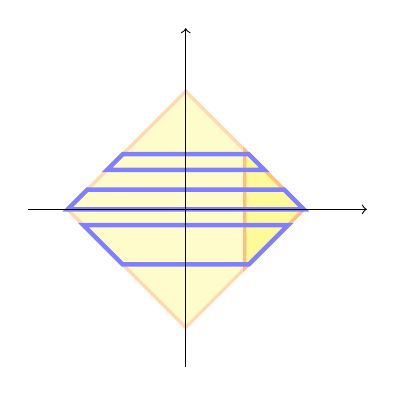
\begin{tikzpicture}
    \filldraw[color=orange!30, fill=yellow!20, very thick] (-1.5, 0)--(0, 1.5)--(1.5, 0)--(0, -1.5)--cycle;
    \filldraw[very thick, color=orange!50, fill=yellow!40] (1.5, 0)--(0.75, 0.75)--(0.75, -0.75)--cycle;
    \draw[color=blue!50, ultra thick] (-1.5, 0)--(1.5, 0)--(1.25, 0.25)--(-1.25, 0.25)--cycle;
    \draw[color=blue!50, ultra thick] (1, 0.5)--(-1, 0.5)--(-0.8, 0.7)--(0.8, 0.7)--cycle;
    \draw[color=blue!50, ultra thick] (-1.3, -0.2)--(1.3, -0.2)--(0.8, -0.7)--(-0.8, -0.7)--cycle;
    \draw[->] (0, -2)--(0, 2.3);
    \draw[->] (-2, 0)--(2.3, 0);
  \end{tikzpicture}\end{center}

  Niech $C\in\sigma(Y)$ takie, że $C=\{Y\in B\}$ dla $B\in Bor(\R)$ (niebieskie kształty na obrazku). Wtenczas
  \begin{align*}
    \expected{\prob{2X>1}{Y}\mathds{1}_C}&=\prob{\{2X>1\}\cap C}=\\ 
                                         &=\prob{\{2X>1\;i\;Y\in B\}}=\\ 
                                         &=\int_{B\cap [0, 1/2]}\int_{1/2}^{1-y}\frac{1}{2}dxdy+\int_{B\cap[-1/2, 0)}\int_{1/2}^{1+y}\frac{1}{2}dxdy=\\ 
                                         &=\frac{1}{2}\int_{B\cap [0, 1/2]}\left[\frac{1}{2}-y\right]dy+\frac{1}{2}\int_{B\cap[-1/2, 0)}\left[{\frac{1}{2}+y}\right]dy
  \end{align*}

  Czyli
  $$\prob{2X>1}{Y}=\frac{1}{2}\begin{cases}\frac{1}{2}-Y & Y\in[0, \frac{1}{2}]\\ \frac{1}{2}+Y & Y\in[-\frac{1}{2}, 0)\\ 0 & wpp.\end{cases}=h(Y),$$
  bo dla $C$ jak wyżej
  \begin{align*}
    \expected{h(Y)\mathds{1}_C}&=\expected{h(Y)\mathds{1}_{B\cap [0, 1/2]}}+\expected{h(Y)\mathds{1}_{B\cap[-1/2, 0)}}=\\ 
                               &=\frac{1}{2}\int_{B\cap [0, 1/2]}({1/2-y}) dy + \frac{1}{2}\int_{B\cap [-1, 0)}({1/2+y})dy
  \end{align*}

  [najmniej pewny fragment rozwiązania ahead]

  Próbując interpretować to geometrycznie, widać, że $2X>1$ tylko jeśli $Y\in[-1/2, 1/2]$. Dalej, jeśli ustalimy sobie jakiegoś dowolnego $Y$ z tego przedziału, to odległość od bliższego ogranicznika tego obszaru wynosi $\frac{1}{2}-Y$, jeśli $Y\geq 0$. Mnożąc to przez $2$ dostalibyśmy pole całego takiego paska: $[-1, 1]\times [Y, 1/2]$. Natomiast mnożąc przez $\frac{1}{2}$ dostajemy pole paska $[1/2, 1]\times[Y, 1/2]$.
  %stosunek długości kreski równoległej do $OX$ na wysokości tego $Y$ zachaczającej o $2X>1$ jest 1/4 długości całej kreski:
  \begin{center}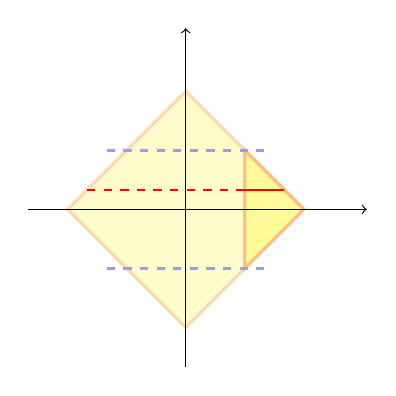
\begin{tikzpicture}
    \filldraw[color=orange!30, fill=yellow!20, very thick] (-1.5, 0)--(0, 1.5)--(1.5, 0)--(0, -1.5)--cycle;
    \filldraw[very thick, color=orange!50, fill=yellow!40] (1.5, 0)--(0.75, 0.75)--(0.75, -0.75)--cycle;
    \draw[->] (0, -2)--(0, 2.3);
    \draw[->] (-2, 0)--(2.3, 0);
    \draw[dashed, very thick, blue!40] (1, 0.75)--(-1, 0.75);
    \draw[dashed, very thick, blue!40] (1, -0.75)--(-1, -0.75);
    \draw[red, thick, dashed] (0.75, 0.25)--(-1.25, 0.25);
    \draw[red, thick] (1.25, 0.25)--(0.75, 0.25);
  \end{tikzpicture}\end{center}
  \end{solution}

\newpage

\section{23.10.23 : Interpretacje geometryczne WWO}

Rozważmy zmienną losową $X$ taką, że $\expected{X^2}<\infty$. Interesuje nas zagadnienie regresji, mianowicie obserwując inną zmienną losową $Z$ chcemy móc $X$ aproksymować. Przez przybliżanie $X$ rozumiemy przybliżanie średniokwadratowe. 

Szukamy więc funkcji mierzalnej $h_0:\R\to\R$ takiej, żeby 
$$\expected{(X-h_0(Z))^2}=\inf_{h:\R\to\R}\expected{(X-h(Z))^2}$$

\begin{fact}\label{fakt 3.1}
  Dla każdej zmiennej losowej $Y$ mierzalnej względem $\sigma(Z)$ (co w skrócie będziemy notować $Y\in\sigma(Z)$) istnieje $h$ takie, że $Y=h(Z)$.
\end{fact}

\begin{proof}
  Zadanie, moja próba poniżej.

  Zaczynamy od $Y$ będącego funkcją prostą i przechodzimy do coraz to bardziej skomplikowanych postaci funkcji mierzalnych.

  Jeżeli $Y=\mathds{1}_A$, to ponieważ $Y$ jest $\sigma(Z)$-mierzalne, mamy $A\in\sigma(Z)$. To znaczy, że istnieje $B\in Bor(\R)$ taki, że $Z(A)=B$, czyli $A=Z^{-1}[B]$ i wówczas
  $$Y=\mathds{1}_A=\mathds{1}_{Z^{-1}[B]}=\mathds{1}_B(Z)$$

  Zrobimy tutaj jeszcze krok $Y=\sum a_i\mathds{1}_{A_i}$. Dla każdego $i$ wiemy, że $\mathds{1}_{A_i}=h_i(Z)$, gdyż są to funkcje $\sigma(Z)$-mierzalne. W takim razie:
  $$Y=\sum a_i\mathds{1}_{A_i}=\sum a_i\cdot h_i(Z)=\left[\sum a_i\cdot h_i\right](Z)$$
  a więc szukane $h=\sum a_i\cdot h_i$.

  Teraz załóżmy, że istnieje ciąg funkcji prostych $s_1\leq s_2\leq...\leq Y$ taki, że $Y=\lim s_i$. Wówczas pokazaliśmy już, że każda funkcja $s_i=h_i(Z)$ dla pewnego borelowskiego $h_i:\R\to\R$. Ciąg $s_i$ jest zbieżny, więc również ciąg $h_i$ musi zbiegać do pewnego $h$. Wówczas dla dowolnego $\omega\in\Omega$
  $$Y(\omega)=\lim s_i(\omega)=\lim h_i(Z(\omega))=h(Z(\omega))$$
  czyli $Y=h(Z)$ dla $h=\lim h_i$.

  Dla formalności należy rozważyć jeszcze $Y=Y^+-Y^-$, gdzie $Y^+$ oraz $Y^-$ podlegają pod poprzedni podpunkt.
\end{proof}

$$\expected{(X-h(Z))^2}=\inf_{Y\in\sigma(Z)}\expected{(X-Y)^2}$$
mając pewną wiedzę o przestrzeniach Hilberta jest do tego dość naturalne podejście: rzut ortogonalny.

Dla $\sigma$-ciała $\set{G}\subseteq\set{F}$ będziemy rozważać
$$L^2(\set{G})=\{Y\in\set{G}\;:\;\expected{Y^2}<\infty\}$$
wówczas $L^2(\set{G})$ jest przestrzenią Euklidesową z iloczynem skalarnym $\langle X, Y\rangle=\expected{XY}$, który z kolei zadaje normę
$$\|X\|=\sqrt{\expected{X^2}}.$$

Używając tego języka będziemy wiedzieli jak szukać $Y$ z początku wykładu, ale najpierw fakt pomocniczy do twierdzenia które nadejdzie lada moment.

\begin{fact}[warunkowa wersja nierówności Cauchy'ego-Schwartza]\label{warunkowy Cauchy-szwarc}
  Dla zmiennych  $X,Y$ takich, że $\expected{X^2},\expected{Y^2}<\infty$ i $\sigma$-ciała $\set{G}\subseteq\set{F}$ zachodzi
  $$\expected{|XY|}{\set{G}}\leq\expected{X^2}{\set{G}}^{\frac{1}{2}}\expected{Y^2}{\set{G}}^{\frac{1}{2}}$$
\end{fact}

\begin{proof}
  Zadanie, tutaj moje podejście.


  Zauważmy na początku, że
  $$XY=\underbrace{\frac{(\expected{Y^2}{\set{G}}+\frac{1}{n})^{1/4}}{(\expected{X^2}{\set{G}}+\frac{1}{n})^{1/4}}X}_{X_n}\underbrace{\cdot\frac{(\expected{X^2}{\set{G}}+\frac{1}{n})^{1/4}}{(\expected{Y^2}{\set{G}}+\frac{1}{n})^{1/4}}Y}_{Y_n}$$
  przy czym korzystamy z $\frac{1}{n}$, żeby na pewno nie dzielić przez $0$ gdy np. $\expected{X^2}{\set{G}}=0$.

  Dalej zauważmy, że ponieważ $(X_n-Y_n)^2\geq0$, to również
  $$0\leq\expected{(X_n-Y_n)^2}{\set{G}}=\expected{X_n^2+Y_n^2-2X_nY_n}{\set{G}}$$
  czyli korzystając z liniowości i przenosząc $\expected{X_nY_n}{\set{G}}$ na lewą stronę nierówności dostajemy
  \begin{align*}\expected{XY}{\set{G}}&={\color{blue}
    \expected{X_nY_n}{\set{G}}\leq 
  \frac{1}{2}\expected{X_n^2}{\set{G}}+\frac{1}{2}\expected{Y_n^2}{\set{G}}}=\\ 
  &=\frac{1}{2}\expected{\frac{(\expected{Y^2}{\set{G}}+\frac{1}{n})^{1/2}}{(\expected{X^2}{\set{G}}+\frac{1}{n})^{1/2}}X^2}{\set{G}}+\frac{1}{2}\expected{\frac{(\expected{X^2}{\set{G}}+\frac{1}{n})^{1/2}}{(\expected{Y^2}{\set{G}}+\frac{1}{n})^{1/2}}Y^2}{\set{G}}=(\heartsuit)
  \end{align*}
  a ponieważ $\frac{(\expected{Y^2}{\set{G}}+\frac{1}{n})^{1/2}}{(\expected{X^2}{\set{G}}+\frac{1}{n})^{1/2}}$ jest $\set{G}$-mierzalne, to możemy wyciągnąć je przed nawias:
  \begin{align*}
    (\heartsuit)&=\frac{1}{2}\cdot \frac{ (\expected{Y^2}{\set{G}}+\frac{1}{n})^{1/2}}{ (\expected{X^2}{\set{G}}+\frac{1}{n})^{1/2}} \expected{X^2}{\set{G}}+\frac{1}{2}\cdot  \frac{ (\expected{X^2}{\set{G}}+\frac{1}{n})^{1/2}}{ (\expected{Y^2}{\set{G}}+\frac{1}{n})^{1/2}} \expected{Y^2}{\set{G}}\to\\ 
                &\xrightarrow{n\to\infty}(\expected{Y^2}{\set{G}})^{1/2}(\expected{X^2}{\set{G}})^{1/2}
  \end{align*}
\end{proof}

Z tego nierówności w fakcie \ref{warunkowy Cauchy-szwarc} wynika, że dla $Y=1$ mamy
$$\expected{|X|}{\set{G}}^2\leq\expected{X^2}{\set{G}}\implies\expected{\expected{X}{Y}^2}<\infty$$

\begin{theorem}[wwo jest rzutem ortogonalnym na $L^2(\set{G})$]
  Niech $X$ będzie zmienną losową taką, że $\expected{X^2}<\infty$, a $\set{G}\subseteq\set{F}$ jest $\sigma$-ciałem. Wówczas 
  $$\expected{X}{\set{G}}\in L^2(\set{G})$$
  jest \acc{rzutem ortogonalnym} $X$ na $L^2(\set{G})$.
\end{theorem}

\begin{center}\begin{tikzpicture}
  \node (X) at (0, 3) {$X$};
  \filldraw (0, 2.7) circle (1.5pt);

  \filldraw (-2, 0) circle (1.5pt);
  \node (0) at (-2, -0.3) {$0$};
  
  \filldraw (0, 0);
  \draw(-2, 0)--(0, 2.7);
  \draw[dashed](0, 2.7)--(0, 0);

  %\draw (-3, 1.5) rectangle (3, -1.5);
  %\draw plot[smooth, tension=2] coordinates {(-3, -2) (3, -1.5)};
  \draw (-3, 1.5) to[out=-20,in=220] (3, 2);
  \draw (3, 2) to[out=5, in=5] (3, -2);
  \draw (3, -2) to[out=150, in=20] (-3, -1.5);
  \draw (-3, -1.5) to[out=170, in=200] (-3, 1.5);

  \node at (2.7, -1) {$L^2(\set{G})$};
\end{tikzpicture}\end{center}

Dokładniej, $\expected{X}{\set{G}}$ daje minimum zbioru $\{\expected{(X-Y)^2}\;:\;Y\in L^2(\set{G})\}$. Z faktu \ref{fakt 3.1} dla $\set{G}=\sigma(Z)$, $\expected{X}{\set{G}}=h_0(Z)$ dla pewnego $h_0$.

\begin{proof}
  Dla $Y\in L^2(\set{G})$ mamy 
  \begin{align*}
    \expected{(X-Y)^2}&=\expected{((X-\expected{X}{\set{G}})-\overbrace{(Y-\expected{X}{\set{G}})}^{=Y'})^2}=\\
                      &=\expected{(X-\expected{X}{\set{G}})^2}-2\expected{(X-\expected{X}{\set{G}})Y'}+\expected{(Y')^2}=\\
                      &\overset{\star}{=}\expected{(X-\expected{X}{\set{G}})^2}+\expected{(Y')^2}
  \end{align*}
  Zauważmy, że
  \begin{align*}\expected{Y'X}{\set{G}}&=Y'\expected{X}{\set{G}}\\
    \expected{\expected{Y'X}{\set{G}}}=\expected{Y'X}&=\expected{Y'\expected{X}{\set{G}}}
\end{align*}
\end{proof}

\begin{example}
  \item Niewiele mający z tym co przed chwilą było. Niech $\Omega=[0,1]$, $\set{F}=Bor([0,1])$ i $\prob=\lambda$. Chcemy rozważyć $t\in(0,1)$ oraz $\set{G}=\sigma(Bor([0,t])$.

    Dla całkowalnej zmiennej losowej $X$ szukamy $\expected{X}{\set{G}}$.

    Dowolny $G\in\set{G}$ ma postać $G=A\cup B$, gdzie $A\in Bor([0, t])$ i $B\in \{(t, 1],\emptyset\}$. W takim razie, jeśli $Y\in \set{G}$, to $Y$ jest stała na $(t, 1]$. Czyli żeby $Y=\expected{X}{\set{G}}$ to zapewne będzie postaci:
    $$Y(\omega)=X(\omega)\mathds{1}_{[0, t]}(\omega)+c\mathds{1}_{(t, 1]}(\omega)$$
      gdzie $c$ jest pewną stałą.

      Musimy sprawdzić, czy (i kiedy) $\expected{X\mathds{1}_G}=\expected{Y\mathds{1}_{G}}$. Widać od razu, że dla $G=A\cup B$ jak wyżej, mamy
      $$X\mathds{1}_A=Y\mathds{1}_A,$$
      czyli $\expected{X\mathds{1}_A}=\expected{Y\mathds{1}_A}$. Zostaje nam uzgodnić część $B$ kiedy jest on niepusty:
      $$\expected{X\mathds{1}_B}=\int_t^1X(s)ds$$
      $$\expected{Y\mathds{1}_B}=c(1-t),$$
      czyli $c$ musi być średnią $X$ na przedziale $(t, 1]$:
      $$c=\frac{1}{1-t}\int_t^1X(s)ds.$$
\end{example}

\subsection{Regularne rozkłady warunkowe}

Dla zmiennej losowej $Y$ i całkowalnej zmiennej losowe $X$ napis
$$\expected{X}{Y}:=\expected{X}{\sigma(Y)}$$
będzie wwo $X$ względem $\sigma$-ciała generowanego przez $Y$.


\textbf{Zadanie dla dociekliwych:}

Jeśli $\prob{Y=y}>0$ dla $y\in\R$, to biorąc $\omega\in\{Y=y\}$ dostajemy:
$$\expected{X}{Y}(\omega)=\expected{X}{Y=y}=\frac{1}{\prob{Y=y}}\expected{X\mathds{1}_{\{Y=y\}}}$$

\begin{definition}[wwo $X$ pod warunkiem $\{Y=y\}$]
 Po pierwsze zauważamy, że istnieje funkcja $h:\R\to\R$ taka, że $\expected{X}{Y}=h(Y)$. ($\star$)

  Niech $X$ i $Y$ będą dowolnymi zmiennymi losowymi, przy czym od $X$ wymagamy całkowalności. Dla $y\in\R$ warunkową wartość oczekiwaną $X$ pod warunkiem $\{Y=y\}$ definiujemy przez 
  $$\expected{X}{Y=y}=h(y)$$
  gdzie $h$ spełnia warunek ($\star$).
\end{definition}

Podobnie definiujemy prawdopodobieństwo zbioru $A$ pod warunkiem $\{Y=y\}$:
$$\prob{A}{Y=y}=\expected{\mathds{1}_A}{Y=y}$$

\begin{example}
\item Jeżeli $X$ i $Z$ są niezależne, to chcemy zapytać o
  $$\prob{X+Z\in B}{X=x}\overset{?}{=}\prob{Z+x\in B}=\mu_Z(B-x)$$

  Wysławiając tę wartość w terminach całego $X$:
  \begin{align*}
    \prob{X+Z\in B}{X}&=\expected{\mathds{1}_{X+Z\in B}}{X}\overset{\star}{=}\expected{\phi(X, Z)}{X}=\Phi(X)
  \end{align*}
  w $\star$ definiujemy: $\phi(x,z)=\mathds{1}_{x+z\in B}$. Dla ustalonego $x$ mamy więc:
  $$h(x)=\expected{\phi(x, Z)}=\expected{\mathds{1}_{x+Z\in B}}=\prob{Z+x\in B}$$
\item Niech wektor losowy $(X, Y)$ ma gęstość łączną $f(x,y)$. Wówczas
  $$\prob{X\in B}{Y=y}=\int_Bf_{X|Y}(x,y)dx,$$
  gdzie 
  $$f_{X|Y}(x,y)=\frac{f(x,y)}{\int f(t,y)dt}.$$
\item Rozważmy $\prob{E_1\in\bullet}{E_1+E_2=y}$ dla $E_1,E_2$ niezależnych o rozkładzie $Exp(1)$.

  Przyłożymy do tego przypadku wzór z przykładu 2. Wektor losowy $(E_1, E_1+E_2)$ ma rozkład losowy o łącznej gęstości $f(x, y)=e^{-x}e^{-(y-x)}\mathds{1}_{y\geq x\geq0}$. 
  $$\int f(s, y)ds=\int_0^ye^{-y}ds=y,$$
  czyli 
  $$f_{E_1|E_1+E_2}(x, y)=\frac{1}{y}\mathds{1}_{y\geq x\geq 0}$$
  co daje rozkład jednostajny:
  $$\prob{E_1\in\bullet}{E_1+E_2=y}=U[0, y](\bullet)$$
\end{example}
\bigskip

Można zadać sobie pytanie, czy
$$\prob{A}{Y=y}=\expected{\mathds{1}_A}{Y=y}$$
zawsze zadaje miarę probabilistyczną? Okazuje się, że tak faktycznie jest.

\begin{definition}[regularny rozkład warunkowy]
  Niech $X$ będzie zmienną losową, a $\set{G}\subseteq\set{F}$ będzie $\sigma$-ciałem. Funkcja 
  $$\kappa_{X,\set{G}}:\Omega\times Bor(\R)\to [0,1]$$
  nazywa się \buff{regularnym rozkładem warunkowym} [rrw] $X$ pod warunkiem $\set{G}$, jeżeli
  \begin{itemize}
    \item[(R1)] Dla każdego $B\in Bor(\R)$ zmienna losowa $\kappa_{X,\set{G}}(\bullet, B)$ jest $\set{G}$-mierzalna
    \item[(R2)] Dla każdej $\omega\in\Omega$ $\kappa_{X,\set{G}}(\omega,\bullet)$ jest rozkładem prawdopodobieństwa na prostej.
    \item[(R3)] Dla każdego $B\in Bor(\R)$ i $\prob$-p.w. $\omega\in\Omega$
      $$\prob{X\in B}{\set{G}}(\omega)=\kappa_{X,\set{G}}(\omega, B)$$
  \end{itemize}
\end{definition}

\begin{theorem}[rrw istnieje]
  Dla każdego $X$ i dla każdego $\set{G}$ istnieje rrw $X$ pod warunkiem $\set{G}$
\end{theorem}

\begin{proof}
  W notatkach
\end{proof}

\begin{fact}\label{fakt 3.5}
  Dla funkcji $f:\R\to\R$ i zmiennej losowej $X$ takiej, że $\expected{|f(X)|}<\infty$ mamy
  $$\expected{f(X)}{\set{G}}(\omega)=\int_{\R} f(x)\kappa_{X,\set{G}}(\omega,dx)$$
\end{fact}

Pisząc to mówię "weź $f(x)$ i weź miarę $\kappa$ w punkcie $\omega$ i scałkuj $\kappa$".

\begin{proof}
  Ćwiczenia.

  Będziemy przechodzić od najprostszych możliwych funkcji $f$ do coraz to bardziej skomplikowanych konstrukcji.

  W pierwszych kroku niech $f(x)=\mathds{1}_B(x)$ dla $B\in Bor(\R)$. Wówczas 
  \begin{align*}
  \expected{f(X)}{\set{G}}(\omega)&=\expected{\mathds{1}_B(X)}{\set{G}}(\omega)=\expected{\mathds{1}_{\{X\in B\}}}{\set{G}}(\omega)=\\ 
                                  &=\prob{X\in B}{\set{G}}(\omega)=\kappa_{X,\set{G}}(\omega, B)=\\ 
                                  &=\int_B\kappa_{X,\set{G}}(\omega, dx)=\int_{\R} \mathds{1}_B(x)\kappa_{X,\set{G}}(\omega, dx)
  \end{align*} 

  Dalej, niech $f(x)=\sum a_i\mathds{1}_{A_i}(x)$. Wtedy mamy
  \begin{align*}
    \expected{f(X)}{\set{G}}(\omega)&=\expected{\sum a_i\mathds{1}_{A_i}(X)}{\set{G}}(\omega)=\sum a_i\expected{\mathds{1}_{A_i}(X)}{\set{G}}(\omega)=\\ 
                                    &=\sum a_i\int_{\R}\mathds{1}_{A_i}(x)\kappa_{X,\set{G}}(\omega, dx)=\int_{\R}\sum a_i\mathds{1}_{A_i}(x)\kappa_{X,\set{G}}(\omega, dx)=\\ 
                                    &=\int_{\R}f(x)\kappa_{X,\set{G}}(\omega, dx)
  \end{align*}

  Teraz niech $f(x)=\lim s_i(x)$ dla $0\leq s_1\leq s_2\leq...\leq f$ dla prostych funkcji $s_i$ jak z poprzednich podpunktów. Zauważmy, że mamy tutaj predyspozycje do skorzystania z twierdzenia o zbieżności monotonicznej.
  \begin{align*}
    \expected{f(X)}{\set{G}}(\omega)&=\expected{\lim s_i(X)}{\set{G}}(\omega)=\lim\expected{s_i(X)}{\set{G}}(\omega)=\\ 
                            &=\lim \int_{\R} s_i(x)\kappa_{X,\set{G}}(\omega, dx)=\int_{\R}\lim s_i(x)\kappa_{X,\set{G}}(\omega, dx)=\\ 
                            &=\int_{\R}f(x)\kappa_{X,\set{G}}(\omega, dx)
  \end{align*}

  Ostatni krok w dowodzie to $f=f^+-f^-$ i korzysta się tutaj już tylko z poprzednich podpunktów oraz liniowości wwo:
  \begin{align*}
    \expected{f(X)}{\set{G}}(\omega)&=\expected{f^+(X)-f^-(X)}{\set{G}}(\omega)=\expected{f^+(X)}{\set{G}}(\omega)-\expected{f^-(X)}{\set{G}}(\omega)=\\ 
                            &=\int_{\R}f^+(x)\kappa_{X,\set{G}}(\omega, dx)-\int_{\R}f^-(x)\kappa_{X,\set{G}}(\omega, dx)=\\ 
                            &=\int_{\R}(f^+(x)-f^-(x))\kappa_{X,\set{G}}(\omega, dx)=\int_{\R}f(x)\kappa_{X,\set{G}}(\omega, dx)
  \end{align*}
\end{proof}

Jeżeli $G=\sigma(Z)$, to pojęcie rrw troszkę się upraszcza (z naciskiem na trochę):

\begin{definition}
  Dla zmiennych losowych $X,Y$ funkcję $\kappa_{X,Y}:\R\times Bor(\R)\to[0,1]$ nazywamy rrw $X$ pod warunkiem $Y$, jeżeli:
  \begin{itemize}
    \item[(P1)] Dla każdego $B\in Bor(\R)$ funkcja $\kappa_{X,Y}(\bullet, B)$ jest borelowska
    \item[(P2)] Dla każdego $y\in\R$, $\kappa_{X,Y}(y,\bullet)$ jest rozkładem prawdopodobieństwa na prostej.
    \item[(P3)] $\prob{X\in B}{Y=y}=\kappa_{X,Y}(y, B)$
  \end{itemize}
\end{definition}


\subsection{Zadania}

\setcounter{problem}{0}

\begin{problem}
  Niech $Y$ i $Z$ będą dowolnymi zmiennymi losowymi. Pokaż, że jeżeli zmienna $Y$ jest $\sigma(Z)$-mierzalna, to istnieje borelowska funkcja $h:\R\to \R$ taka, że $Y=h(Z)$.
\end{problem}

\begin{solution}
  Treść dowodu faktu \ref{fakt 3.1}.
\end{solution}

\begin{problem}
  Pokaż, że dla zmiennych $X$ i $Y$ takich, że $\expected{X^2},\expected{Y^2}<\infty$ i $\sigma$-ciała $\set{G}\subseteq\set{F}$ zachodzi
  $$|\expected{XY}{\set{G}}|\leq[\expected{X^2}{\set{G}}]^{1/2}[\expected{Y^2}{\set{G}}]^{1/2}$$
\end{problem}

\begin{solution}
  Patrz dowód twierdzenia \ref{warunkowy Cauchy-szwarc}.
\end{solution}

\begin{problem}
  Niech $\kappa_{X,\set{G}}$ będzie regularnym rozkładem warunkowym $X$ pod warunkiem $\sigma$-ciała $\set{G}\subseteq\set{F}$. Pokaż, że dla każdej funkcji $f:\R\to\R$ takiej, że $\expected{|f(X)|}<\infty$ zachodzi
  $$\expected{f(X)}{\set{G}}(\omega)=\int_{\R}f(x)\kappa_{X,\set{G}}(\omega,dx)$$
\end{problem}

\begin{solution}
  Kolejne rozwiązanie jako dowód faktu \ref{fakt 3.5}.
\end{solution}

\begin{problem}
  (Nierówność Jensena) Dana jest funkcja wypukła $\phi:\R\to\phi$, przestrzeń probabilistyczna $(\Omega,\set{F},\prob)$ oraz $\set{G}$ pod-$\sigma$-ciało $\set{F}$. Załóżmy, że zmienne losowe $X$ i $\phi(X)$ są całkowalne. Pokaż, że
  $$\phi(\expected{X}{\set{G}})\leq\expected{\phi(X)}{\set{G}}$$
\end{problem}

\begin{solution}
  Korzystając z faktu \ref{fakt 3.5} możemy powiedzieć, że
  \begin{align*}
    \expected{\phi(X)}{\set{G}}(\omega)&=\int_{\R}\phi(x)\kappa_{X,\set{G}}(\omega, dx)\geq\\ 
                                       &\geq\phi\left[\int_{\R}\kappa_{X,\set{G}}(\omega, dx) \right]=\phi(\expected{X}{\set{G}})
  \end{align*}
  nierówność wynika z twierdzenia Jensena dla całek (które mówi, że $\int \phi\circ f\;d\mu\geq\phi\left(\int f\;d\mu\right)$) a ostatnie przejście to ponowne zastosowanie faktu \ref{fakt 3.5}, tym razem dla $\expected{id(X)}{\set{G}}$.
\end{solution}

\begin{problem}
  Załóżmy, że wektor losowy $(X,Y)$ ma dwuwymiarowy rozkład normalny.
  \begin{enumerate}[label=(\alph*)]
    \item Znajdź $a\in\R$ takie, że zmienne $X-aY$ i $Y$ są niezależne.
    \item Pokaż, że 
      $$\expected{X}{Y}(\omega)=\mu_X+\frac{Cov(X,Y)}{Var(Y)}(Y(\omega)-\mu_Y),$$
      gdzie $\mu_X=\expected{X}$ oraz $\mu_Y=\expected{Y}$.
    \item Dla $y\in\R$ znajdź rozkład $X$ pod warunkiem $Y=y$.
  \end{enumerate}
\end{problem}

\begin{solution}$ $\vspace{0pt}

  \begin{enumerate}[label=(\alph*)]
    \item Z Rachunku Prawdopodbieństwa 1R wiemy, że jeśli wektor losowy ma rozkład normalny, a jego poszczególne elementy są nieskorelowane, to są one również niezależne. Patrzymy więc na kowariancję
      \begin{align*}
        Cov(X-aY, Y)&=Cov(X, Y)-aCov(Y, Y)=Cov(X, Y)-aVar(Y)
      \end{align*}
      i przyrównujemy ją do $0$
      $$0=Cov(X, Y)-aVar(Y)\implies a=\frac{Cov(X,Y)}{Var(Y)}$$
    \item Zauważmy, że korzystając z poprzedniego punktu możemy przepisać równość jako
      $$\expected{X}{Y}(\omega)=\expected{X}-a\expected{Y}+aY(\omega)=\expected{X-aY}+a\expected{Y}{Y}$$
      gdzie $Y=\expected{Y}{Y}$, bo $Y$ jest $\sigma(Y)$-mierzalne.
      
      Kolejne przekształcenia dają
      $$\expected{X}{Y}-a\expected{Y}{Y}=\expected{X-aY}$$
      co jest prawdą, gdyż po skorzystaniu z liniowości wwo po lewej stronie mamy
      $$\expected{X-aY}{Y}=\expected{X-aY}$$
      a ponieważ $X-aY$ dobraliśmy tak, żeby było niezależne od $Y$, to jest ono również niezależne od $\sigma(Y)$. Czyli wwo jest równe wartości oczekiwanej $X-aY$.
    \item Rozkład $X$ pod warunkiem $Y=y$ to $\kappa_{X,Y}(y,B)=\prob{X\in B}{Y=y}$. Wiemy, że
      $$\prob{X\in B}{Y=y}=\frac{\prob{X\in B\;i\;Y=y}}{\prob{Y=y}}$$
      czyli można wydedukować, że szukamy
      $$\prob{X}{Y=y}=f_{X|Y=y}(x, y)=\frac{f(x, y)}{f_Y(y)}$$
      co jest zbyt dużą liczbą brzydkich obliczeń żeby nawet mi się chciało to dokładnie spisywać. Wystarczy podstawić pod gęstość $(X, Y)$ na górze i do gęstości $Y$ na dole.
  \end{enumerate}
\end{solution}

\newpage

\section{30.10.23 : Martyngały}

Mają coś współnego z jazdą konną (podobno).

\begin{example}
  \item Rozważmy dowolną grę i dla uproszczenia niech polega ona na rzucaniu monetą, na której orzeł wypada z $\prob = p \in (0,1)$. Obstawiamy według zasady double or nothing:
    \begin{itemize}
      \item jeśli wypada orzeł, to podwajamy nasz kapitał
      \item jeżeli wypada reszka, to tracimy wszystko
    \end{itemize}
    Czy taka gra jest sprawiedliwa?

    Rozważmy ciąg niezależnych zmiennych losowych $\{\xi_k\}_{k\in\N}$ o tym samym rozkładzie
    $$\prob{\xi_k=2}=1-\prob{\xi_k=0}=p.$$
    Wówczas ciąg
    $$X_n=\xi_n\cdot\xi_{n-1}\cdot...\cdot\xi_1\cdot X_0$$
    reprezentuje stan konta po $n$-tym rzucie, gdzie $X_0$ to jakaś stała.

    Rozważmy $\sigma$-ciało $\set{F}_n=\sigma(\xi_n,...,\xi_1,X_0)$ generowane przez pierwszych $n$ rzutów i stan początkowy. Zadajmy sobie teraz pytanie, ile wynosi
    $$\expected{X_{n+1}}{\set{F}_n}?$$

    Mamy zależność rekurencyjną $X_{n+1}=\xi_{n+1}X_n$, stąd możemy powiedzieć, że
    $$\expected{X_{n+1}}{\set{F}_n}=\expected{\xi_{n+1}X_n}{\set{F}_n}$$
    samo $X_n$ jest w $\set{F}_n$, więc możemy je wyciągnąć przed $\expected$. Dodatkowo, $\xi_{n+1}$ jest niezależne od $\set{F}_n$, więc
    $$\expected{X_{n+1}}{\set{F}_n}=X_n\expected{\xi_{n+1}}{\set{F}_n}=X_n\expected{\xi_{n+1}}=(2p)\cdot X_n$$

    \begin{itemize}
      \item Jeżeli $p>\frac{1}{2}$, to wówczas
        $$\expected{X_{n+1}}{\set{F}_n}\geq X_n$$
        i wtedy taka gra jest korzystna, bo z coraz to kolejnym rzutem oczekiwania rosną.
      \item Jeżeli $p<\frac{1}{2}$, to wówczas
        $$\expected{X_{n+1}}{\set{F}_n}\leq X_n$$
        i gra jest korzystna, ale dla kasyna a nie gracza.
      \item Jeżeli $p=\frac{1}{2}$, to wówczas
        $$\expected{X_{n+1}}{\set{F}_n}=X_n$$
        i w takim przypadku powiemy, że gra jest sprawiedliwa.
    \end{itemize}
\end{example}

Ten ostatni, uczciwy przypadek to jest jeden ze sposobów, na które możemy myśleć o martyngałach.

\begin{definition}[o martyngałach słów kilka]$ $

  \begin{itemize}
    \item Wstępującą rodzinę $\sigma$-ciał
      $$\mathds{F}=\{\set{F}_n\}_{n\in\N},$$
      $\set{F}_n\subseteq \set{F}_{n+1}$, nazywamy \buff{filtracją}
    \item Powiemy, że ciąg zmiennych losowych $\{X_n\}_{n\in\N}$ jest \buff{$\mathds{F}$-adaptowalny}, jeżeli $X_n\in\set{F}_n$.
    \item Adaptowalny i całkowalny ciąg $\{X_n\}$ nazywamy \acc{nadmartyngałem}, jeśli
      $$\expected{X_{n+1}}{\set{F}_n}\leq X_n$$
    \item Adaptowalny i całkowalny ciąg $\{X_n\}$ nazywamy \acc{podmartyngałem}, jeśli
      $$\expected{X_{n+1}}{\set{F}_n}\geq X_n$$
    \item Z kolei ciąg $\{X_n\}$ jest \buff{martyngałem}, jeśli jest jednocześnie nadmartyngałem i podmartyngałem, czyli zachodzi równość
      $$\expected{X_{n+1}}{\set{F}_n}= X_n$$
  \end{itemize}
\end{definition}

\begin{example}
\item Niech $\{\eta_k\}_{k\in\N}$ będą niezależne takie, że $\expected{\eta_k}=0$ dla każdego $k\in\N$. Wówczas jako filtrację możemy rozważyć
  $$\set{F}_n=\sigma(\eta_1,...,\eta_n)$$
  a jako nowy ciąg zmiennych losowych zdefiniujemy jako $M_0=0$ i 
  $$M_n=\sum_{k=1}^n\eta_k.$$
  Tak zdefiniowany ciąg $\{M_n\}$ jest $\mathds{F}=\{\set{F}_n\}$-martyngałem:
  \begin{align*}
    \expected{M_{n+1}}{\set{F}_n}&=\expected{\eta_{n+1}+M_n}{\set{F}_n}=\\
                                 &=\expected{\eta_{n+1}}{\set{F}_n}+\expected{M_n}{\set{F}_n}=\\
                                 &=\expected{\eta_{n+1}}+M_n=0+M_n=M_n
  \end{align*}
\item Dla dowolnej filtracji $\mathds{F}=\{\set{F}_n\}$ i całkowalnej zmiennej losowej $X$ rozważmy
  $$M_n=\expected{X}{\set{F}_n}.$$
  Wówczas
  $$\expected{M_{n+1}}{\set{F}_n}=\expected{\expected{X}{\set{F}_{n+1}}}{\set{F}_n}=\expected{X}{\set{F}_n}=M_n$$
\end{example}

\begin{uwaga}
  Jeżeli $\{X_n\}$ jest martyngałem, to 
  $$\expected{X_{n+1}}{\set{F}_n}=X_n$$
  czyli mam dwie zmienne losowe które są sobie równe, czyli
  $$\expected{X_{n+1}}=\expected{\expected{X_{n+1}}{\set{F}_n}}=\expected{X_n}$$
  W szczególności, jeśli zastosujemy indukcję, to dostaniemy, że dla dowolnego $n\in\N$
  $$\expected{X_n}=\expected{X_0}$$
\end{uwaga}

\begin{example}\label{procel galtona-watsona}
\item \buff{Proces Galtona-Watsona}

  Rozważmy populację, w której osobniki rozmnażają się bezpłciowo, niezależnie od siebie. Można myśleć o tym jako o obserwacji populacji pantofelków z pomiarami w jakiś określonych odstępach czasu.

  Myślimy o tym jako o drzewie, w którym liczba krawędzi z danego wierzchołka oznacza liczbę potomstwa, a ilość wierzchołków na danej głębokości oznacza ilość pantofelków po $n$-tym pokoleniu.

  \begin{center}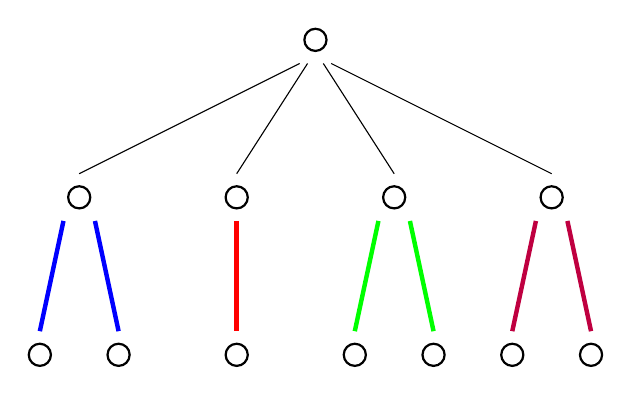
\begin{tikzpicture}
    \draw[thick] (0, 0) circle (4pt);

    \draw (-0.2, -0.3)--(-3, -1.7);
    \draw (-0.1, -0.3)--(-1, -1.7);
    \draw (0.1, -0.3)--(1, -1.7);
    \draw (0.2, -0.3)--(3, -1.7);

    \draw[thick] (-3, -2) circle (4pt);
    
    \draw[blue, ultra thick] (-3.2, -2.3)--(-3.5, -3.7);
    \draw[blue, ultra thick] (-2.8, -2.3)--(-2.5, -3.7);

    \draw[thick] (-3.5, -4) circle (4pt);
    \draw[thick] (-2.5, -4) circle (4pt);


    \draw[thick] (-1, -2) circle (4pt);

    \draw[red, ultra thick] (-1, -2.3)--(-1, -3.7);


    \draw[thick] (-1, -4) circle (4pt);


    \draw[thick] (1, -2) circle (4pt);

    \draw[green, ultra thick] (0.8, -2.3)--(0.5, -3.7);
    \draw[green, ultra thick] (1.2, -2.3)--(1.5, -3.7);

    \draw[thick] (0.5, -4) circle (4pt);
    \draw[thick] (1.5, -4) circle (4pt);


    \draw[thick] (3, -2) circle (4pt);

    \draw[purple, ultra thick] (2.8, -2.3)--(2.5, -3.7);
    \draw[purple, ultra thick] (3.2, -2.3)--(3.5, -3.7);

    \draw[thick] (2.5, -4) circle (4pt);
    \draw[thick] (3.5, -4) circle (4pt);  
  \end{tikzpicture}\end{center}

  Niech $\mu$ będzie dowolnym rozkładem prawdopodobieństwa na $\N=\{0,1,...\}$. Rozważmy zmienne losowe losowe indeksowane parami liczb naturalnych $\{Y_{n,k}\}_{n,k\in\N}$. Kładziemy 
  $$Z_1=1$$
  $$Z_{n+1}=\sum_{k=1}^{Z_n}Y_{n+1,k}$$
  $Z_1$ to liczba pantofelków na samym początku, $Z_2=Y_{2,1}$ to liczba dzieci pierwszego pantofelka, z kolei
  $$Z_3={\color{blue}Y_{3,1}}+{\color{red}Y_{3,2}}+{\color{green}Y_{3,3}}+{\color{purple}Y_{3,4}},$$
  co odpowiada kolorom na rysunku. To znaczy, że $Y_{n+1,k}$ to liczba potomstwa w generacji $n+1$ zrodzona z $k$-tego pantofelka w generacji $n$.

  Filtracją będzie dla nas ciąg o elementach $\set{F}_n=\sigma(Y_{j,k}\;:\;k\in\N,j\leq n)$. Chcemy zapytać się o wartość oczekiwaną $Z_{n+1}$
  \begin{align*}
    \expected{Z_{n+1}}{\set{F}_n}&=\expected{\sum^{Z_n}_{k=1}Y_{n+1,k}}{\set{F}_n}=h(Z_n)
  \end{align*}
  gdzie 
  $$h(z)=\expected{\sum_{k=1}^zY_{{n+1},k}}=z\cdot \underbrace{\expected{Y_{n,k}}}_{m}=m\cdot z,$$
  bo wszystkie $Y_{n,k}$ mają taką samą średnią. Oznacza to, że
  $$\expected{Z_{n+1}}{\set{F}_n}=m\cdot Z_n.$$
  Jeżeli $m< 1$, to dostajemy w ten sposób nadmartyngał, jeśli $m> 1$ to mamy podmartyngał, a w krytycznym przypadku $m=1$, to $\{Z_n\}$ jest martyngałem.

  Jeśli pomnożymy
  $$\expected{Z_{n+1}}{\set{F}_n}=mZ_n$$
  oboma stronami przez $m^{-n-1}$, to dostajemy
  $$\expected{m^{-n-1}Z_{n+1}}{\set{F}_n}=m^{-n}Z_n$$
  i wtedy $W_n=m^{-n}Z_n$ jest zawsze martyngałem, bo
  $$\expected{W_{n+1}}{\set{F}_n}=W_n$$
\end{example}

\subsection{Transformata martyngałowa}

Stan konta gracza wynosi $X_n$ po $n$-tej sprawiedliwej grze. Przychodzi drugi gracz i obstawia on wyniki w grze tego pierwszego. Wypłata drugiego gracza wynosi $B_n\cdot (X_n-X_{n-1})$, tzn. za każdy przychód pierwszego gracza dostaje jakąś część tej wygranej.

Dla ciągu funkcji $B_n\in\set{F}_{n+1}=\sigma(X_0,...,X_{n-1})$. Żeby było łatwiej, niech drugi gracz zaczyna z tym samym kapitałem co pierwszy. Stan konta drugiego gracza po $n$-tej grze wynosi 
$$W_n=\sum_{k=1}^nB_k\cdot(X_k-X_{k-1})+X_0.$$
Tak zdefiniowany ciąg $\{Q_n\}$ jest również martyngałem, bo
\begin{align*}
  \expected{W_{n+1}}{\set{F}_n}&=\expected{B_{n+1}\cdot(X_{n+1}-X_n)}{\set{F}_n}+\expected{W_n}{\set{F}_n}=\\
                               &=B_{n+1}\expected{X_{n+1}-X_n}{\set{F}_n}+W_n=\\
                               &=B_{n+1}(\expected{X_{n+1}}{\set{F}_n}-X_n)+W_n=W_n
\end{align*}
bo $X_n$ sam w sobie był martyngałem, więc $X_n=\expected{X_{n+1}}{\set{F}_n}$.

\begin{definition}
  Niech $\mathds{F}$ będzie filtracją. Zmienną losową $T:\Omega\to \N\cup\{+\infty\}$ nazywamy \buff{$\mathds{F}$-czasem zatrzymania}, jeżeli zdarzenie $\{T=n\}$ jest mierzalne względem $\set{F}_n$ dla każdego $n\in\N$.
\end{definition}

\begin{example}
\item Rzucamy $10$-krotnie monetą. Zdefiniujmy zmienną losową
  $$X_n=\begin{cases}1&\text{orzeł w n-tym}\\0&wpp\end{cases}$$
  Filtracją niech będzie $\set{F}_n=\sigma(X_1,...,X_n)$. Jeśli $T$ będzie momentem wypadnięcia pierwszego orła, a $S$ - wypadnięcia ostatniego orła, to $T$ jest czasem zatrzymania, bo
  $$\{T=n\}=\{X_1=0,X_2=0,...,X_n=1\}\in\set{F}_n$$
  a $S$ nim nie jest, bo wymaga informacji wybiegającej w przyszłość:
  $$\{S=n\}=\{X_n=1,X_{n+1}=0,....\}\notin\set{F}_n$$
\item Rozważmy $\mathds{F}$-adaptowalny ciąg zmiennych losowych $\{X_n\}$. Dla $B\in Bor(\R)$ kładziemy 
  $$T(B)=\inf\{n\;:\;X_n\in B\}.$$
  Tak zdefiniowane $T$ jest czasem zatrzymania:
  $$\{T=n\}=\{X_1\notin B,...,X_{n-1}\notin B,X_n\in B\}\in\set{F}_n$$
\item Jeżeli $T=n_0$ dla pewnego $n_0\in\N$, to taka stała funkcja nadal jest czasem zatrzymania, bo
  $$\{T=n\}=\begin{cases}\emptyset&n\neq n_0\\\Omega&n=n_0\end{cases}$$
\end{example}


\subsection{Zadania}

\setcounter{problem}{0}

\begin{problem}
  Załóżmy, że $\{X_n\}_{n\in\N}$ jest ciągiem niezależnych zmiennych losowych o takim samym rozkładzie, średniej $0$ i skończonej wariancji. Rozważmy filtrację $\mathds{F}=\{\set{F}_n\}$ zadaną przez $\set{F}_n=\sigma(X_0,X_1,...,X_n)$. Udowodnij, że ciąg
  $$Z_n=X_0X_1+X_1X_2+....+X_{n-1}X_n, \quad Z_0=0$$
  jest $\mathds{F}$-martyngałem.
\end{problem}

\begin{solution}
  Chcemy pokazać, że
  $$\expected{Z_{n+1}}{\set{F}_{n}}=Z_n$$
  dla dowolnego $n\in\N$.
  \begin{align*}
    \expected{Z_{n+1}}{\set{F}_n}&=\expected{Z_n+X_nX_{n+1}}{\set{F}_n}=\\ 
                                 &=\expected{Z_n}{\set{F}}+\expected{X_nX_{n+1}}{\set{F}_n}=\\ 
                                 &=Z_n+X_n\expected{X_{n+1}}{\set{F}_n}
  \end{align*}
  ponieważ $X_n$ jest $\set{F}_n$-mierzalne oraz
  $$\expected{|X_nX_{n+1}|}\leq\expected{X_n^2}^{1/2}\expected{X_{n+1}^2}^{1/2}<\infty$$
  gdzie nierówność wynika z nierówności Cauchy'ego-Schwarza, a $\expected{X_n^2}=Var(X_n)<\infty$.

  Zauważmy teraz, że $X_{n+1}$ jest niezależne od $\set{F}_n$, gdyż $X_n$ jest niezależne od każdej ze zmiennych $X_1,...,X_n$. W takim razie, $\expected{X_{n+1}}{\set{F}_n}=\expected{X_{n+1}}=0$, a więc ostatecznie dostajemy
  $$\expected{Z_{n+1}}{\set{F}_n}=Z_n+X_n\expected{X_{n+1}}{\set{F}_n}=Z_n+X_n\cdot 0=Z_n$$
  Czyli $Z_n$ faktycznie jest martyngałem.
\end{solution}

\begin{problem}
  Ustalmy $\theta\in\R$. Niech $X_1,X_2,...$ będzie ciągiem niezależnych zmiennych losowych o takim samym rozkładzie takich, że 
  $$\expected{e^{\theta X_1}}<\infty.$$
  Pokaż, że 
  $$M_n=\expected{e^{\theta X_1}}^{-n}\prod_{j=1}^ne^{\theta X_j}$$
  jest $\mathds{F}$-martyngałem dla filtracji $\mathds{F}=\{\set{F}_n\}$ danej przez $\set{F}_n=\sigma(X_1,...,X_n)$.
\end{problem}

\begin{solution}
  Zacznijmy od obserwacji, że
  $$M_{n+1}=\expected{e^{\theta X_1}}^{-n-1}\prod_{j=1}^{n+1}e^{\theta X_j}=M_n\cdot\expected{e^{\theta X_1}}^{-1}e^{\theta X_{n+1}}$$
  w takim razie, wwo $M_{n+1}$ to jest
  \begin{align*}
    \expected{M_{n+1}}{\set{F}_n}&=\expected{e^{\theta X_1}}^{-1}\cdot \expected{M_n\cdot e^{\theta X_{n+1}}}{\set{F}_n}
  \end{align*}
  Od razu widać, że $M_n$ jest mierzalne względem $\set{F}_n$, bo zależy tylko od zmiennych $X_1,...,X_n$ które $\set{F}_n$ generują. Chcemy teraz sprawdzić, czy $\expected{|M_n\cdot e^{\theta X_{n+1}}|}<\infty$, wówczas możemy wyciągnąć $M_n$ przed wwo.
  \begin{align*}
    \expected{|M_n\cdot e^{\theta X_{n+1}}|}&=\expected{\left |\expected{e^{\theta X_1}}^{-1}\cdot \prod_{j=1}^{n} e^{\theta X_j}\cdot e^{\theta X_{n+1}} \right| }=\\ 
                                            &=|\expected{e^{\theta X_1}}|^{-n}\cdot\expected{ \prod_{j=1}^{n+1}e^{\theta X_j} }=\\ 
                                            &=|\expected{e^{\theta X_1}}|^{-n}\cdot \prod_{j=1}^{n+1}\expected{e^{\theta X_j}}=\\ 
                                            &=\expected{e^{\theta X_{n+1}}}=\expected{e^{\theta X_1}}<\infty
  \end{align*}
  ponieważ jeśli $\{X_n\}$ są niezależne, to $e^{X_n}$ też są niezależne, a dla niezależnych $X,Y$ zachodzi $\expected{XY}=\expected{X}\expected{Y}$.
  W takim razie dostajemy
  $$\expected{M_{n+1}}{\set{F}_n}=\expected{e^{\theta X_1}}^{-1}\expected{M_n\cdot e^{\theta X_{n+1}}}{\set{F}_n}=M_n\expected{e^{\theta X_1}}^{-1}\expected{e^{\theta X_{n+1}}}{\set{F}_{n}}$$
  ale ponieważ $\set{F}_n$ nie zawiera ani grama informacji o $X_{n+1}$, to $e^{\theta X_{n+1}}$ jest niezależne od $\set{F}_n$, więc
  $$\expected{e^{\theta X_{n+1}}}{\set{F}_n}$$
    a to już daje to co chcieliśmy.
\end{solution}

\newpage

\section{06.11.23 : Twierdzenie Dooba o zatrzymaniu, czyli jak uprawiać hazard}

%\begin{definition}
  Dla $T:\Omega\to\N$ i procesu $\{X_n\}$ definiujemy zmienną $X_T$ wzorem
  $$X_T(\omega)=X_{T(\omega)}(\omega)$$

  Dla martyngału $\{X_n\}_{n\in\N}$ i czasu zatrzymania $T$ rozważamy ciąg zmiennych $\{X_{n\land T}\}_{n\in\N}$
  $$\color{blue}X_{n\land T}(\omega)=\begin{cases}X_n& n\leq T(\omega)\\ X_{T(\omega)}(\omega) & n\geq T(\omega) \end{cases}$$
%\end{definition}

  Tutaj dla $X,y\in\R$ piszemy $x\land y$ aby przekazać, że interesuje nas $\min\{x,y\}$. To znaczy $x\land y=\min\{x,y\}$.

Czyli gramy w pewna uczciwą grę i mamy strategię wyjścia $T$, ale musimy np. zdążyć na obiad, więc chcemy wyjść po co najwyżej $n$ rundach.

\begin{theorem}[Dooba o zatrzymaniu (uproszczone)]
  Niech $\{X_n\}$ będą odpowiednio martyngałem i czasu zatrzymania względem tej samej filtracji $\mathds{F}=\{\set{F}_n\}$. Wówczas proces (ciąg) $\{X_{n\land T}\}$ zdefiniowany wyżej jest martyngałem. W szczególności
  $$\expected{X_{n\land T}}=\expected{X_0}$$
  dla każdego $n$ (średnia jest stała w czasie).
\end{theorem}

\begin{proof}
  Mamy 
  $$X_{n\land T}=\sum_{k=1}^{n\land T}(X_k-X_{k-1})+X_0=\sum_{k=1}^n\mathds{1}_{T\geq k}(X_k-X_{k-1})+X_9$$
  gdzie
  $$\mathds{1}_{T\geq k}=1-\mathds{1}_{T<k}=1-1_{T\leq k-1}\in \set{F}_{k-1}$$
  i teza wynika z przykładu o transformacie martyngałowej.
\end{proof}

\begin{example}
  \item Gracz rozpoczyna grę z kapitałem $j\$$. W każdym rozdaniu może z prawdopodobieństwem $\frac{1}{2}$ zyskać jednego dolara lub go stracić. Celem gracza jest wzbogacenie się o $k$ dolarów. Jakie jest prawdopodobieństwo sukcesu $p_{k,j}$?

    Zaczynamy w punkcie $j$ i chcemy dojść do punktu $j+k$, a boimy się punktu $0$

    \begin{center}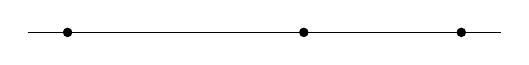
\begin{tikzpicture}
      \draw (-0.5, 0)--(5.5, 0);
      \filldraw (0, 0) circle (1.5pt);
      \filldraw (5, 0) circle (1.5pt);
    \filldraw(3, 0) circle (1.5pt);
    \end{tikzpicture}\end{center}

    Niech $\{\xi_k\}$ będą niezależne o tym samym rozkładzie $\prob{\xi_k=\pm 1}=\frac{1}{2}$. Rozważmy
    $$X_n=\sum_{k=1}^n\xi_n.$$
    Żeby rozwiązać to zadanie to chcemy rozważyć funkcję
    $$T=\inf\{n\in\N\;:\; X_n=-j\text{ lub }X_n=k\}$$
    Teraz szukane przez nas prawdopodobieństwo to
    $$p_{k,j}=\prob{X_T=k}$$

    Rozważamy filtrację $\mathds{F}=\{\set{F}_n\},\; \set{F}_n=\sigma(\xi_1,...,\xi_n)$. Ciąg $\{X_n\}$ jest $\mathds{F}$-adaptowalny, więc $T$ jest $\mathds{F}$-czasem zatrzymania.

    Ciąg $\{X_n\}$ jest $\mathds{F}$-martyngałem, co wynika z faktu, że $\xi_{n+1}$ są niezależne od $\set{F}_n$ i mają $\expected$ równą $0$:
    $$\expected{X_{n+1}}{\set{F}_n}=\expected{\xi_{n+1}+X_n}{\set{F}_n}=\expected{\xi_{n+1}}+\expected{X_n}{\set{F}_n}=0+X_n$$
    Z twierdzenia o zatrzymaniu wiemy więc, że
    $$\expected{X_{n\land T}}=\expected{X_0}=0$$
    i tutaj szkopuł jest taki, że nas interesuje $X_T$ a nie $X_{n\land T}$. Musimy więc przejść z $n$ do nieskończoności.

    W pierwszej kolejności chcemy się upewnić, że $\prob{T<\infty}=1$, bo 
    $$\prob{T\geq n}\leq \prob{|X_n|\leq k+j}=\prob{\frac{|X_n|}{\sqrt{n}}\leq \frac{j+k}{\sqrt{n}}}\xrightarrow{CTG} 0$$
    a ponieważ
    $$\prob{T=\infty}=\lim_{n\to\infty}\prob{T\geq n}=0.$$
    W takim razie ciąg $X_{n\land T}$ zbiega prawie wszędzie do ciągu $X_T$. Mało tego, dla pewnego $n$ się zacznie stabilizować. Pozostaje uzasadnić, że możemy wejść z granicą pod całkę, ale to wynika z faktu, że
    $$|X_{n\land T}|\leq j+k,$$
    więc mamy
    $$0=\expected{X_0}=\lim \expected{X_{n\land T}}=\expected{\lim X_{n\land T}}=\expected{X_T}.$$
    Rozpisując już na końcu
    \begin{align*}
      0=\expected{X_T}&=k\prob{X_T=k}-j\prob{X_T=-j}=k\cdot p_{k,j}-j(1-p_{k,j})
    \end{align*}
    co pozwala nam wyliczyć
    $$p_{k,j}=\frac{j}{k+j}.$$

    W szczególności mamy
    \begin{align*}
      \prob{\{X_n\}\text{ osiągnie k}}&=\lim_{j\to\infty}\prob{\{X_k\}\text{ osiągnie k przed osiągnięciem -j}}=\\ 
                                      &=\lim_{j\to\infty}p_{k,j}=\lim_{j\to\infty}\frac{j}{j+k}=1
    \end{align*}
  \item Gracz rozpoczyna grę z kapitałem $j\$$. W każdym rozdaniu może z prawdopodobieństwem $p$ zyskać jednego dolara lub stracić go z prawdopodobieństwem $(1-p)$. Celem gracza jest wzbogacenie się o $k$ dolarów. Jakie jest prawdopodobieństwo sukcesu $p_{k,j}$ gdy $p>\frac{1}{2}$?

    Jest to niemalże takie samo zadanie jak wcześniej, z tym że tym razem nie mamy martyngału. Niemniej jednak modelować będziemy to w niemalże identyczny sposób.

    Niech $\{\eta_k\}$ będą iid takie, że $\prob{\eta_k=1}=p$ oraz $\prob{\eta_k=-1}=1-p$. Określamy $X_n=\sum_{k=1}^n\eta_k$. Mamy wówczas
    \begin{align*}
      \expected{X_{n+1}}{\set{F}_n}&=\expected{\eta_{n+1}}+X_n=X_n+(2p-1)>X_n
    \end{align*}
    czy $\{X_n\}$ jest podmartyngałem. Określmy czas zatrzymania
    $$T=\inf\{n\;:\;X_n=-j\text{ lub }X_n=k\}.$$

    Chcemy sobie zorganizować nowy martyngał postaci
    $$M_n=f(X_n)$$
    dla pewnej funkcji $f:\Z\to\R$ takiej, że
    $$\expected{M_{n+1}}{\set{F}_n}=M_n.$$
    Mamy
    \begin{align*}
      \expected{M_{n+1}}{\set{F}_n}&=\expected{f(X_n+\eta_{n+1}}{\set{F}_n}=\\ 
                                   &=F(X_n),
    \end{align*}
    gdzie $F(x)=\expected{f(x+\eta_{n+1})}=pf(x+1)+(1-p)f(x-1)$ jest oznaczeniem pomocniczym przy "odcałkowaniu niezależnej $\eta_{n+1}$".

    Aby $\{M_n\}$ był martyngałem musi zachodzić
    $$M_n=f(X_n)=pf(X_n+1)+(1-p)f(X_n-1)=F(X_n)=\expected{M_{n+1}}{\set{F}_n}$$
    $f$ musi zatem spełniać rekurencję
    $$f(x)=pf(x+1)+(1-p)f(x-1)$$
    Szukamy rozwiązania postaci $f(x)=\gamma^x$. Mamy więc
    $$\gamma^x=p\gamma^{x+1}+(1-p)\gamma^{x-1}$$
    $$\gamma=p\gamma^2+(1-p)$$
    i istnieją dwa rozwiązania: $\gamma=1$ oraz $\gamma=\frac{1-p}{p}$. Wówczas
    $$M_n=f(X_n)=\left(\frac{1-p}{p}\right)^{X_n}$$
    jest martyngalem. Znowu $M_{n\land T}\leq\left(\frac{p}{1-p}\right)^{k+j}$, a z twierdzenia Dooba
    $$\expected{M_{n\land T}}=\expected{M_0}=1$$
    i poprzez przejście graniczne
    $$\expected{M_T}=1$$
    Oznaczamy $\prob{X_T=k}=r_{j,j}$ i mamy
    $$1=\expected{M_T}=\gamma^{-j}(1-r_{k,j})+\gamma^kr_{k,j}$$
    gdzie
    $$r_{k,j}=\frac{1-\gamma^{-j}}{\gamma^k-\gamma^{j-1}}$$
    w szczególności
    $$\prob{\{X_n\}\text{ osiągnie k}}=\lim_{j\to\infty} r_{j,k}=1$$
    $$\prob{\{X_n\}\text{ osiągnie j}}=\lim_{k\to\infty}(1-r_{k,j})=\lim_{k\to\infty}...=\gamma^j$$

  \item Rozważmy $X_n=\sum Y_k$, gdzie $Y_k$ są iid takie, że $\prob{Y_1=\pm 1}=\frac{1}{2}$. To znaczy, że jeden gracz bierze udział w uczciwej grze i obstawiamy.
\end{example}


\subsection{Zadania}
\setcounter{problem}{0}

\begin{problem}
  Uzasadnij, że jeżeli $\{X_n\}$ są niezależnymi całkowalnymi zmiennymi losowymi o tym samym rozkładzie, a $T$ jest czasem zatrzymania względem filtracji $\set{F}_n=\sigma(X_1,...,X_n)$, takim że $\expected{T}<\infty$, to 
  $$\expected{S_T}=\expected{T}\cdot\expected{X_1}$$
  gdzie $S_n=X_1+X_2+...+X_n$.
\end{problem}

\begin{solution}
  PLAN:
  \begin{center}\scalebox{0.7}{
    \begin{tikzpicture}
      \node (a1) at (0, 0) {martyngał $Y_n=S_n-n\expected{X_1}$};
      \node (a2) at (0, -1.5) {$T$ jest prawie wszędzie skończony};
      \node (a3) at (0, -3) {$Y_{n\land T}$ od pewnego momentu jest stale równy $Y_T$}; 
      \node (a4) at (0, -4.5) {granica $\expected{\lim Y_{n\land T}}=\lim\expected{Y_{n\land T}}$ ma sens};
      \node (a5) at (0, -6) {$\expected{Y_T}=\expected{S_T-T\expected{X_1}}=0$};

      \draw[->] (a1)--(a2);
      \draw[->] (a2)--(a3);
      \draw[->] (a3)--(a4);
      \draw[->] (a4)--(a5);
  \end{tikzpicture}}
  \end{center}

  Jesteśmy w temacie martyngałów, więc możemy chcemy tego użyć.

  Niech $m=\expected{X_1}=\expected{X_n}$ dla każdego $n$. Dobrym początkiem będzie pokazanie, że ciąg $\{S_n-nm\}$ jest martyngałem. W tym celu potrzebujemy całkowalności $[S_n-nm]$, $\set{F}_n$-mierzalności i równości wwo.
  \begin{enumerate}
    \item $[S_n-nm]$ jest całkowalne
    $$\expected{|S_n-nm|}=\expected{\left|\sum X_k-m\right|}\leq\expected{\sum|X_k-m|}=\sum\expected{|X_k-m|}<\infty$$
  \item $[S_n-nm]$ jest $\set{F}_n$-mierzalne, bo jest skończoną sumą $\set{F}_n$-mierzalnych funkcji (wraz z funkcją stałą).
    \item $\expected{S_{n+1}-(n+1)m}{\set{F}_n}=S_n-nm$
      \begin{align*}
        \expected{S_{n+1}-(n+1)m}{\set{F}_n}&=\expected{\sum^{n+1} (X_i-m)}{\set{F}_n}=\\ 
                                            &=\expected{X_{n+1}-m}{\set{F}_n}+\sum(X_i-m)=\\ 
                                            &=\expected{X_{n+1}}-m+S_n-nm=m-m+S_n-nm=S_n-nm
      \end{align*}
  \end{enumerate}

  Dla uładnienia zapisu niech $Y_k=n=S_n-n\cdot m$, wtedy $\{Y_n\}$ jest martyngałem względem filtracji jak w zadaniu. 
  Z twierdzenia Dooba o zatrzymaniu wiemy, że
  $$\expected{Y_{n\land T}}=\expected{Y_1}=S_1-m=0$$
  Będziemy chcieli przejść z $n$ do granicy, do czego potrzebujemy aby $\prob{T\geq n}\to 0$, bo wówczas ciąg $X_{n\land T}$ zbiega prawie wszędzie do $X_T$. Wystarczy przypomnieć sobie ostatnie zadanie z poprzedniej listy, aby dostać
  $$\expected{T}=\sum_{k\geq 0}\prob{T>k}<\infty$$
  czyli w pewnym momencie wyrazu muszą być dowolnie blisko $0$, czyli faktycznie $\prob{T\geq n}\to 0$.

  Przechodząc z $n$ do granicy dostajemy
  $$\expected{Y_T}=\expected{\lim Y_{n\land T}}=\lim\expected{Y_T}=0$$
  ponieważ $Y_{n\land T}$ zbiega do $Y_T$, więc od pewnego momentu jest stały i granica ma sens.

  Rozbijając więc $Y_T$ na wzór podany wyżej, dostajemy
  $$0=\expected{Y_T}=\expected{S_T-Tm}=\expected{S_T}-\expected{T\expected{X_1}}$$
  czyli
  $$\expected{S_T}=\expected{T\expected{X_1}}=\expected{X_1}\expected{T}$$
  tak jak chcieliśmy.
\end{solution}

\begin{problem}
  Rzucamy kostką tak długo, aż pięciokrotnie wyrzucimy szóstkę. Znajdź średnią wartość sumy wyrzuconych oczek.
\end{problem}

\begin{solution}
  Zadania wygląda bardzo podobnie jak równość udowadniana wyżej. Chcemy tylko znaleźć martyngał i czas zatrzymania.

  Niech $X_i$ będzie liczbą oczek wyrzuconych w $i$-tym rzucie, a $S_n=\sum_{k=1}^nX_i$ będzie sumą oczek wyrzuconych w pierwszych $n$ rzutach. Oczywiście, $X_i$ mają ten sam rozkład jednostajny na zbiorze $\{1,...,6\}$ i są od siebie niezależne. Zdefiniujmy teraz funkcję
  $$T=\inf \{n\;:\;(X_1,...,X_n)\;\text{posiada 5 szóstek}\}$$
  która jest czasem zatrzymania względem filtracji $\mathds{F}=\{\set{F}_n\}$, $\set{F}_n=\sigma(X_1,...,X_n)$, bo jej definicja opiera się wyłącznie na informacjach o $X_1,...,X_n$.

  Korzystając więc z poprzedniego zadania, dostajemy
  $$\expected{S_T}=\expected{T}\expected{X_1}=\expected{T}\cdot\frac{7}{2}$$
  i jedynym problemem jest obliczenie 
  $$\expected{T}=\sum_{n\geq0}n\prob{T=n}.$$
  Oczywiście, dla $\prob{T=1}=\prob{T=4}=0$, a w pozostałych przypadkach jest to stosunek wszystkich ciągów długości $n-1$ które posiadają dokładnie $4$ szóstki do ilości wszystkich ciągów posiadających co najwyżej $4$ szóstki.
\end{solution}

\begin{problem}
  Niech $\{X_n\}$ będzie niesymetrycznym spacerem losowym na $\Z$ (tzn. $X_n=\sum_{k=1}^n\xi_k$, gdzie $\xi_k$ są iid takie, że $\prob{\xi_k=1}=1-\prob{\xi_k=-1}=p\neq\frac{1}{2}$) i niech $T=\min\{n\;:\;X_n=-j\text{ lub }X_n=k\}$ dla ustalonych $k,j>0$.
  \begin{enumerate}[label=(\alph*)]
    \item Pokaż, że $M_n=X_n+n(1-2p)$ jest martyngałem.
    \item Wykorzystując twierdzenie Dooba oblicz $\expected{T}$.
  \end{enumerate}
\end{problem}

\begin{solution}$ $
  Filtrem u mnie będzie $\set{F}_n=\sigma(\xi_1,...\xi_n)$.

  \begin{enumerate}[label=(\alph*)]
    \item Wypadałoby pokazać, że $M_n$ jest całkowalne, czyli
      \begin{align*}
        \expected{|M_n|}&=\expected{|X_n+n(1-2p)|}\leq \expected{|X_n|}+n(1-2p)=\\ 
                        &=\expected{|\sum\xi_k|}+n(1-2p)\leq \sum\expected{|\xi_k|}+n(1-2p)<\infty 
      \end{align*}
      Jest $\set{F}_n$-mierzalne bo jest kombinacją funkcji $\set{F}_n$-mierzalnej z funkcją stałą. Pozostaje warunek z wwo:
      \begin{align*}
        \expected{M_{n+1}}{\set{F}_n}&=\expected{X_{n+1}+(n+1)(1-2p)}{\set{F}_n}=\\ 
                                     &=\expected{X_{n+1}}{\set{F}_n}+(n+1)(1-2p)=\\ 
                                     &=\expected{\sum^{n+1}\xi_k}{\set{F}_n}+(n+1)(1-2p)=\\ 
                                     &=\sum^{n+1}\expected{\xi_k}{\set{F}_n}+(n+1)(1-2p)=\\ 
                                     &=X_n+n(1-2p)+\expected{\xi_{n+1}}{\set{F}_n}+(1-2p)=\\ 
                                     &=X_n+n(1-2p)=M_n
      \end{align*}
    \item To jest tak samo jak w zadaniu $1$, tylko trzeba pokazać, że z prawdopodobieństwem $1$ w kończenie wielu krokach dojdziemy do $-j$ lub $k$. A tutaj można użyć Borel-Cantalliego :3
  \end{enumerate}
\end{solution}

\begin{problem}
  Niech $\{M_n\}$ będzie nieujemnym martyngałem. Pokaż, że dla $m>n$, $\{M_n=0\}\subseteq\{M_m=0\}$ prawie wszędzie.
\end{problem}

\begin{solution}
  Rozważmy zbiór $A=\{M_n=0\}\in\set{F}_n$. Ponieważ $\{M_n\}$ jest martyngałem, to na poprzedniej liście pokazywaliśmy, że
  $$\expected{M_m}{\set{F}_n}=M_n.$$
  W takim razie mamy
  \begin{align*}
    0=\expected{M_n\mathds{1}_A}=\expected{\expected{M_m}{\set{F}_n}\mathds{1}_A}=\expected{M_m\mathds{1}_A}
  \end{align*}
  Ponieważ $M_m\geq0$ oraz $\int_AM_md\prob=0$, to $M_m=0$ prawie wszędzie na zbiorze $A$. Czyli 
  $$A\subseteq\{M_m=0\}$$ 
  prawie wszędzie.

  %  Rozważmy zmienną losową
%  $$T=\inf\{n\;:\;(\forall\;k\geq n)\;M_k=0\}$$
%
%
%  Rozważmy zbiór
%  $$A=\{\omega\;:\;M_n(\omega)\neq 0\;i\;M_m(\omega)=0\}$$
%  chcemy pokazać, że $\prob{A}=0$.
%
%  Zauważmy, że $A$ zawiera informacje o $\omega$ pojawiające się tylko w $\sigma(M_1,...,M_m)$.
%  \begin{align*}
%    \prob{A}&=\expected{\mathds{1}_A}
%  \end{align*}
\end{solution}

\begin{problem}
  Niech $\mathds{F}=\{\set{F}_n\}$ będzie filtracją.
  \begin{enumerate}[label=(\alph*)]
    \item Pokaż, że dla każdych $m,n\in\N$, $m<n$ i zdarzenia $A\in\set{F}_m$ zmienna losowa
      $$\tau=m+(n-m)\mathds{1}_A$$
      jest $\mathds{F}$-czasem zatrzymania.
    \item Niech $\{X_n\}$ będzie $\mathds{F}$-adaptowalnym ciągiem całkowalnych zmiennych losowych takim, że
      $$\expected{X_\tau}=\expected{X_0}$$
      dla każdego skończonego czasu zatrzymania $\tau$. Pokaż, że $\{X_n\}$ jest $\mathds{F}$-martyngałem.
  \end{enumerate}
\end{problem}

\begin{solution}$ $

  \begin{enumerate}[label=(\alph*)]
    \item Musimy sprawdzić, że zdarzenie $\{\tau=k\}\in\set{F}_k$. Od razu widzimy, że $\tau$ ma jedynie dwie możliwe wartości:
      $$\tau(\omega)=\begin{cases}m & \omega\not\in A\\n & \omega\in A\end{cases}$$
      Zacznijmy od $\{\tau =m\}$. Ale tak jak wyżej napisaliśmy, to zachodzi tylko dla $\omega\not\in A$, czyli $\{\tau=m\}=A^c\in\set{F}_m$, bo $A\in\set{F}_m$.

      Z kolei $\{\tau=n\}=A$, a wiemy, że $A\in\set{F}_m\subseteq\set{F}_n$ bo $m<n$.

      W takim razie $\tau$ zachowuje się jak bardzo dziwny czas zatrzymania.
    \item PLAN na ten podpunkt jest taki (pokazujemy $\expected{X_{m+1}}{\set{F}_m}=X_m$):
      \begin{center}\scalebox{0.6}{
        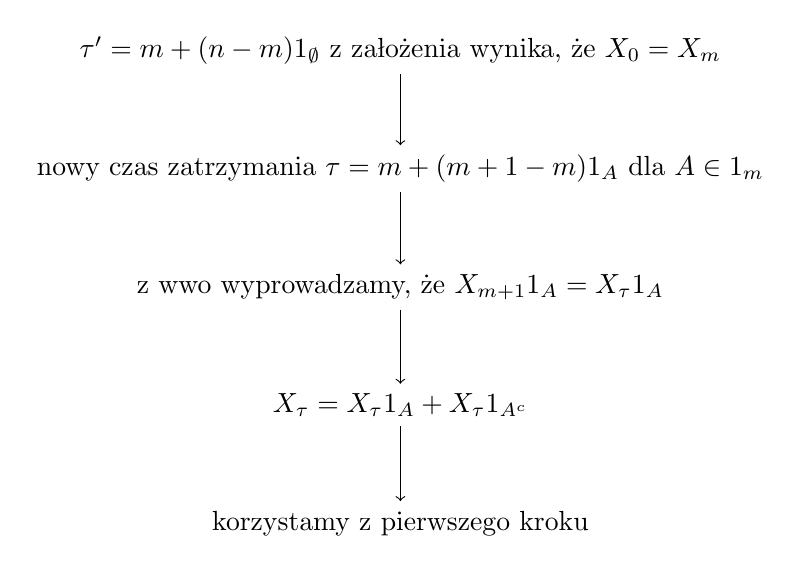
\begin{tikzpicture}
          \node (a1) at (0, 0) {$\tau'=m+(n-m)\mathds{1}_\emptyset$ z założenia wynika, że $\expected{X_0}=\expected{X_m}$};
          \node (a2) at (0, -1.5) {nowy czas zatrzymania $\tau=m+(m+1-m)\mathds{1}_A$ dla $A\in\mathds{1}_m$};
        \node (a3) at (0, -3) {z wwo wyprowadzamy, że $\expected{X_{m+1}\mathds{1}_A}=\expected{X_\tau\mathds{1}_A}$ };
        \node (a4) at (0, -4.5) {$\expected{X_\tau}=\expected{X_\tau\mathds{1}_A}+\expected{X_\tau\mathds{1}_{A^c}}$};
        \node (a5) at (0, -6) {korzystamy z pierwszego kroku};
          \draw[->] (a1)--(a2);
          \draw[->] (a2)--(a3);
          \draw[->] (a3)--(a4);
          \draw[->] (a4)--(a5);
      \end{tikzpicture}}
      \end{center}

      Zaczniemy od wprowadzenia czasu zatrzymania
      $$\tau'=m+(n-m)\mathds{1}_\emptyset$$
      dla dowolnego $n>m$ i użycia założenia z tego punktu, by otrzymać
      $$\expected{X_0}=\expected{X_{\tau'}}=\expected{X_{\tau'}\mathds{1}_\emptyset}+\expected{X_{\tau'}\mathds{1}_{\emptyset^c}}=\expected{X_m\mathds{1}_\Omega}=\expected{X_m}$$
      gdyż $\expected{X_{\tau'}\mathds{1}_\Omega}=\int_\Omega X_{\tau'(\omega)}(\omega)=\int X_m$ - całkujemy tę część tylko po zbiorze gdzie $\tau'=m$.

      Rozważamy teraz czas zatrzymania
      $$\tau=m+(m+1-m)\mathds{1}_A=m+(m+1)\mathds{1}_A$$
      dla dowolnego $A\in\set{F}_m$.

      Z jednej strony wiemy, że
      $$\expected{\expected{X_{m+1}}{\set{F}_m}\mathds{1}_A}=\expected{X_{m+1}\mathds{1}_A}=\expected{X_\tau\mathds{1}_A}$$
      A z drugiej
      $$\expected{X_0}=\expected{X_\tau}=\expected{X_\tau\mathds{1}_A}+\expected{X_\tau\mathds{1}_{A^c}}=\expected{X_{m+1}\mathds{1}_A}+\expected{X_m\mathds{1}_{A^c}}$$
      czyli korzystając z $\expected{X_0}=\expected{X_m}$ mamy
      $$\expected{X_{m+1}\mathds{1}_A}=\expected{X_0}-\expected{X_m\mathds{1}_{A^c}}=\expected{X_m}-\expected{X_m\mathds{1}_{A^c}}=\expected{X_m(1-\mathds{1}_{A^c}}=\expected{X_m\mathds{1}_A}$$
      i to już wystarczy, bo $X_m$ jest mierzalne względem $\set{F}_m$ ponieważ jest $\mathds{F}$-adaptowalne.
  \end{enumerate}
\end{solution}

\begin{problem}
  Niech $\{M_n\}$ będzie nieujemnym martyngałem o wartościach całkowitym takim, że $M_0=m\geq1$, $M_n-M_{n-1}\leq 1$ oraz $M_n\to 0$ p.w.. Pokaż, że dla $k\geq m$,
  $$\prob{\sup_{n\in\N}M_n\geq k}=\frac{m}{k}$$
\end{problem}

\begin{solution}
  Zacznijmy od rozważenia co znaczy, że $\sup_{n\in\N}M_n\geq k$. Moim skromnym zdaniem jest to powiedzenie, że $M_n$ dojdzie do $k$. Wiemy, że w każdym przejściu z $M_n$ do $M_{n+1}$ możemy skoczyć w górę o nie więcej niż $1$, a w dół możemy skakać aż do $0$.

  PLAN na to zadanie jest taki:
  \begin{center}\scalebox{0.6}{
    \begin{tikzpicture}
      \node (a1) at (0, 0) {czas zatrzymania $T=\inf\{n\;:\;M_n\geq k\}$};
      \node (a2) at (0, -1.5) {$\sup{M_n}\geq k\iff T<\infty$, więc $\prob{\sup M_n\geq k}=\prob{T<\infty}$};
      \node (a3) at (0, -3) {twierdzenie Dooba daje $m=\expected{M_0}=\expected{M_{n\land T}}$};
      \node (a4) at (0, -4.5) {$\lim_n M_{n\land T}$ będzie $M_T=k$ jeśli $T<\infty$ i $M_n$ wpp.};
      \node (a5) at (0, -6) {$M_{n\land T}\in\{0,...,k\}$};
      \node (a6) at (0, -7.5) {$\prob{M_{n\land T}<k}\to 0$, bo jeśli $T=\infty$ to $M_n\to 0$, a jeśli $T<\infty$, to $M_{n\land T}\to M_T=k$ jest stałe od pewnego momentu};
      \node (a7) at (0, -9) {$\lim \prob{M_{n\land T}=k}=\prob{T<\infty}$};
      \node (a8) at (0, -10.5) {$m=\sum_{0\leq i\leq k} i\prob{M_{n\land T}}\to k\prob{T<\infty}$};

      \draw[->] (a1)--(a2);
      \draw[->] (a2)--(a3);
      \draw[->] (a3)--(a4);
      \draw[->] (a4)--(a5);
      \draw[->] (a5)--(a6);
      \draw[->] (a6)--(a7);
      \draw[->] (a7)--(a8);
  \end{tikzpicture}}
  \end{center}

  Spróbujmy zobaczyć co się stanie, jeśli wplączemy w to zadanie czas zatrzymania
  $$T=\inf\{n\;:\;M_n\geq k\}$$
  to możemy zauważyć, że 
  $$\prob{\sup_{n\in\N}M_n\geq k}=\prob{T<\infty}=\prob{M_{n\land T}=k}$$
  ponieważ $T<\infty$ oznacza, że zbiór $\{n\;:\;M_n\geq k\}$ jest niepusty.

  Z twierdzenia Dooba wiemy, że
  $$m=\expected{M_0}=\expected{M_{n\land T}}$$
  zauważmy, że jeżeli $T(\omega)<\infty$, to $M_{n\land T}(\omega)=M_{T(\omega)}(\omega)=k$, a jeśli $T(\omega)=\infty$, to $M_{n\land T}(\omega)=M_n(\omega)$. 

  Oznacza to, że jeśli $M_{n\land T}\geq k$, to $M_{n\land T}=k$ i jest od tego momentu funkcją stałą. W takim razie
  $$m=\expected{M_{n\land T}}=\sum_{j=0}^kj\prob{M_{n\land T}=j}=k\cdot\prob{M_{n\land T}=k}+\sum_{j=0}^{k-1}j\prob{M_{n\land T}=j}$$
  przechodząc teraz z $n$ do granicy, albo $M_{n\land T}=k$ albo $M_{n\land T}=M_n$ i w obu przypadkach $\prob{M_{n\land T}=j}=0$ dla $j<k$ (bo $M_n\to 0$). W takim razie, po przejściu do granicy z $n$ zostaje nam
  $$m=k\cdot\prob{\sup_{n\in\N}M_n\geq k}$$
  i to jest to co chcieliśmy.
\end{solution}

\begin{problem}
  Niech $Y_k$ będą iid takie, że $\prob{Y_k\in\{-1,0,1\}}=1$ oraz $\expected{Y_k}=0$. Niech $S_0=0$, $S_n=Y_1+...+Y_n$. Dla $k\in\N$ rozważmy moment zatrzymania
  $$T_{-k}=\inf\{n\;:\;S_n=-k\}.$$
  Znajdź rozkład zmiennej losowej
  $$\sup_{n\leq T_{-k}}S_n$$
\end{problem}

\begin{solution}
  Zmienna losowa
  $$\sup_{n\leq T_{-k}}S_n$$
  pyta, jak wysoko możemy dojść, jeśli zatrzymamy się przy pierwszym dojściu do $-k$.

  Popatrzmy teraz na $\prob{Y_k=1}$. Oznaczając $\prob{Y_k=0}=p$ mamy
  $$0=\expected{Y_k}=\prob{Y_k=1}-\prob{Y_k=-1}$$
  $$\prob{Y_k=1}=\prob{Y_k=-1}=\frac{1-p}{2}$$
\end{solution}

\newpage

\section{18.11.23 : Sobotnia mordęga}

\subsection{Nierówności maksymalne}

Niech $X=\{X_n\}$ będzie $\mathds{F}=\{\set{F}_n\}$ podmartyngałem. Wówczas 
$$\expected{X_{n+1}}{\set{F}_n}\geq X_n$$
dla każdego $n\in\N$.

\begin{theorem}[o zatrzymaniu dla podmartyngałów]\label{zatrzymanie podmartyngałów}
  Jeżeli $X$ jest $\mathds{F}$-podmartyngałem, a $T$ $\mathds{F}$-czasem zatrzymania, to dla każdego $n\in\N$ 
  $$\expected{X_n}\geq\expected{X_{n\land T}}$$
\end{theorem}

\begin{proof}
  Mamy 
  \begin{align*}
    X_n-X_{n\land T}&=\sum_{k=n\land T+1}^n(X_k-X_{k-1})=\sum_{k=1}^n\mathds{1}_{\{k\geq n\land T+1\}}(X_k-X_{k-1})=\\ 
                    &=\sum_{k=1}^n\underbrace{\mathds{1}_{\{k\geq T+1\}}}_{\in\set{F}_{k-1}}(X_k-X_{k-1})
  \end{align*}
  Co z własności martyngału da nam
  \begin{align*}
    \expected{\mathds{1}_{\{k\geq T+1\}}(X_k-X_{k-1})}{\set{F}_{k-1}}=\mathds{1}_{\{k\geq T+1\}}\expected{X_k-X_{k-1}}{\set{F}_{k-1}}\geq 0
  \end{align*}
  Czyli jak zsumujemy rzeczy $\geq0$, to również dostaniemy wartość $\geq0$, tzn.
  $$\expected{X_n-X_{n\land T}}\geq0$$
  i to już kończy dowód.
\end{proof}

\begin{theorem}[nierówność maksymalna słabego typu]\label{max slabego}
  Jeżeli $X$ jest podmartyngałem, to dla każdego $n\in\N$ oraz $\lambda>0$ mamy
  $$\prob{\max_{k=0,...,n}X_k\geq\lambda}\leq \expected{X_n\mathds{1}_{\{\max_{k=0,...,n}X_k\geq \lambda\}}}\leq \expected{|X_n|}$$
  (środkowa nierówność nie jest pamiętana przez zdrowych psychicznie ludzi, ale będzie potrzebna do dowodu następnego dowodu)
\end{theorem}

\begin{proof}
  Wybierzmy czas zatrzymania
  $$\tau=\inf\{k\;:\;X_k\geq\lambda\}.$$

  Z twierdzenia o zatrzymaniu \ref{zatrzymanie podmartyngałów} wiemy, że
  \begin{align*}
  \expected{X_n}&\geq\expected{X_{n\land\tau}}= \expected{\underbrace{X_{n\land\tau}}_{=X_\tau}\mathds{1}_{\{\max  X_k\geq \lambda\}}}+\expected{\underbrace{X_{n\land\tau}}_{=X_n}\mathds{1}_{\{\max X_k<\lambda}\}}=(\star)
  \end{align*}
  nawiasy na dole są bo pierwsza całka jest po zbiorze gdzie już mamy $\max\geq \lambda$, a druga jest po zbiorze gdzie to nigdy nie dojdzie do $\lambda$. Idąc dalej mamy
  \begin{align*}
    \expected{X_n}\geq (\star)&\geq \lambda\prob{\max X_k\geq\lambda}+\expected{X_n\mathds{1}_{\max X_k<\lambda}}
  \end{align*}
  Stad, jeśli przerzucimy $\expected$ na jedną stronę, to dostajemy
  $$\expected{X_n\mathds{1}_{\max X_k\geq \lambda}}\geq \lambda\prob{\max X_k\geq\lambda}$$
\end{proof}

\begin{conclusion}
  Jeżeli $M=\{M_n\}$ jest martyngałem takim, że dla pewnego $p\geq1$
  $$\expected{|M_n|^p}<\infty$$
  dla każdego $n\in\N$, to jeśli zastosuje się nierówność Jensena,
  $$X_n=|M_n|^p$$
  jest podmartyngałem.
\end{conclusion}

\begin{proof}
  \begin{align*}
    \expected{X_{n+1}}{\set{F}_n}&=\expected{|M_{n+1}|^p}{\set{F}_n}\geq\ |\expected{M_{n+1}}{\set{F}_n}|^p=|M_n|^p=X_n
  \end{align*}
\end{proof}

Wówczas mamy
\begin{align*}
  \lambda\prob{\max|M_n|^p\geq\lambda}&\leq\expected{|M_n|^p\mathds{1}_{\{\max |M_k|^p\geq\lambda\}}}
\end{align*}
  Czyli dla $s=\lambda^{1/p}$ dostajemy
  $$\prob{\max |M_k|\geq s}\leq \frac{1}{s^p}\expected{|M_n|^p\mathds{1}_{\{\max |M_k|\geq s\}}}$$

\begin{example}
  \item Nierówność maksymalna Kołmogorowa.

    Niech $\xi_k$ będzie ciągiem niezależnych zmiennych z $\expected{\xi_k}=0$ i $\expected{\xi_k^2}<\infty$, to oznaczając $S_n=\sum_{k\leq n}\xi_k$ wiemy już, że $S_n$ jest martyngałem. Wówczas
    $$\prob{\max |S_k|\geq\epsilon}\leq\frac{1}{\epsilon^2}\expected{S_n^2}=\frac{1}{\varepsilon^2}\sum_{k\leq n}\expected{\xi_j^2}$$
\end{example}

\begin{theorem}[nierówność maksymalna mocnego typu]
  Niech $M=\{M_n\}$ będzie martyngałem takim, że $\expected{|M_n|^p}<\infty$ dla pewnego $p>1$ i wszystkich $n\in\N$, to wtedy
  $$\expected{\max|M_k|^p}\leq\left(\frac{p}{p-1}\right)^p\expected{|M_n|^p}$$
\end{theorem}

\begin{proof}
  Oznaczmy
  $$M_n^*=\max_{k\leq n}|M_k|$$
  Mamy dla $k>0$
  \begin{align*}
    \expected{(M_n^*\land k)^p}&=\expected{\int_0^{M_n^*\land k}ps^{p-1}ds}=\expected{\int_0^k\mathds{1}_{\{M_n^*\geq s\}}ps^{p-1}ds}=\\ 
                               &=\int_0^kps^{p-1}\prob{M_n^*\geq s}ds\leq\int_0^kps^{p-1}\overbrace{\color{blue}\frac{1}{s}\expected{|M_n|\mathds{1}_{\{M_n^*\geq s\}}}}^{\ref{max slabego}}=\\ 
                               &=\expected{|M_n|\int_0^kps^{p-2}\mathds{1}_{\{M_n^*\geq s\}}ds}=\expected{|M_n|\int_0^{k\land M_n^*}ps^{p-2}ds}=\\ 
                               &=\frac{p}{p-1}\expected{|M_n|(M_n^*\land k)^{p-1}}\leq\frac{p}{p-1}\expected{|M_n|^p}^{1/p}\expected{|M_n^*\land k|^{p/(p-1)}}^{(p-1)/p}
  \end{align*}
  Przerzucając potworka z $\frac{p}{p-1}$ na lewą stronę, dostajemy
  $$\expected{(M_n^*\land k)^p}^{1/p}\leq \frac{p}{p-1}\expected{|M_n|^p}^{1/p}$$
  przechodząc z $k$ do nieskończoności. Użycie $k$ było potrzebne przy dzieleniu.
\end{proof}

\begin{theorem}\label{tw 7.5}
  Niech $p>1$. Dla martyngału $\{M_n\}$ następujące warunki są równoważne:
  \begin{enumerate}
    \item $\sup \expected{|M_n|^p}<\infty$
    \item istnieje zmienna losowa $M_\infty$ taka, że $\expected{|M_\infty|^p}<\infty$ i $M_n\to M_\infty$ prawie wszędzie w $L^p$
    \item Istnieje zmienna losowa $M_\infty$ taka, że $\expected{|M_\infty|^p}<\infty$ i $\expected{M_\infty}{\set{F}_n}=M_n$.
  \end{enumerate}
\end{theorem}

\begin{dygresja}
  Zbieżność w $L^p$ oznacza, że $\expected{|M_n-M_\infty|^p}\to 0$ prawie wszędzie.
\end{dygresja}

\begin{proof}
  \begin{itemize}
    \item[$1\implies 2$] Wiemy, że
      $$\sup\expected{M_n^*}^p\leq\sup\expected{|M_n|^p}<\infty,$$
      zatem istnieje $M_\infty$ taka, że $M_n\to M_\infty$. Dla każdego $n\in\N$ mamy
      $$\expected{\max|M_k|^p}\leq\left(\frac{p}{p-1}\right)^p\expected{|M_n|^p}\leq \left(\frac{p}{p-1}\right)^p\sup\expected{|M_k|^p}$$
      przy $n\to\infty$ daje to
      $$\expected{\sup |M_k|^p}\leq\left(\frac{p}{p-1}\right)^p\sup\expected{|M_k|^p}$$
      Mamy
      $$|M_n-M_\infty|^p\leq (|M_n|+|M_\infty|)^p \leq2^p\sup|M_k|^p$$
      z twierdzenia o zbieżności ograniczonej wiemy, że
      $$\lim\expected{|M_n-M_\infty|^p}=\expected{\lim|M_n-M_\infty|^p}=0$$
    \item[$2\implies3$] Chcemy pokazać, że
      $$\expected{M_\infty}{\set{F}_n}=M_n$$
      czyli, że dla każdego $A\in\set{F}_n$
      $$\expected{M_\infty\mathds{1}_A}=\expected{M_n\mathds{1}_A}$$
      Wiemy, że dla każdego $m\in\N$ zachodzi
      $$\expected{M_{n+m}}{\set{F}_n}=M_n$$
      czyli
      $$\expected{M_{n+m}\mathds{1}_A}=\expected{M_n\mathds{1}_A}$$
      przy $m\to \infty$ dostajemy
      $$\left[\expected{(M_\infty-M_{n+m})\mathds{1}_A}\right]^p\leq\expected{|M_\infty-M_{n+m}|^p}]to 0$$
      Skoro więc
      $$\expected{M_{n+m}\mathds{1}_A}\xrightarrow{m\to\infty} \expected{M_\infty\mathds{1}_A}$$
    \item[$3\implies 1$] Z założenia i nierówności Jensena mamy, że
      $$|M_n|^p=|\expected{M_\infty}{\set{F}_n}|^p\leq\expected{|M_\infty|^p}{\set{F}_n}$$
      stąd
      $$\expected{|M_n|^p}\leq\expected{|M_\infty|^p}$$
      w szczególności $\sup\expected{|M_n|^p}\leq\infty$.
  \end{itemize}
\end{proof}

\begin{example}
\item Niech $f:[0,1]\to\R$ będzie funkcją w $L^p$, tzn.:
  $$\int_0^1|f(t)|^pdt<\infty$$
  Dla $n\in\N$ niech $I_k^{(n)}=(k-1)2^{-n}, k2^{-n})$. Niech teraz $f_k^{(n)}=2^n\int_{I_k^{(n)}}f(t)dt$ będzie średnią $f$ na przedziale $I_k^{(n)}$.

  Niech teraz $f^{(n)}:[0,1]\to\R$ będzie dana przez
  $$f^{(n)}(t)=\sum_{k=1}^{2^n}f_k^{(n)}\mathds{1}_{I_k^{(n)}}(t)$$
  Wówczas funkcje $f^{(n)}$ przybliżają $f$ w $L^p[0,1]$, tzn $f^{(n)}\to f$.

  Działamy w przestrzeni z $\Omega=[0,1]$, $\prob=\lambda\restriction[0,1]$. Rozważamy rodzinę  $\set{F}_n=\sigma(I_k^{(n)}\;:\;k=1,...,2^n)$, w której mamy $I_{2k}^{(n+1)}\cup I_{2k-1}^{(n+1)}=I_k^{(n)}$, więc jest ona filtracją. 
  $$\expected{f}{\set{F}_n}=\sum_{k=1}^{2^n}\mathds{1}_{I_k^{(n)}}\expected{f}{I_k^{(n)}}=\sum_{k=1}^{2^n}\mathds{1}_{I_k^{(n)}}f_k^{(n)}$$
  Czyli jesteśmy w 3. punkcie równoważności z twierdzenia wyżej, czyli mamy od razu dane 2, gdzie $M_\infty=f$, $M_n=f^{(n)}$.
\end{example}


\end{document}
